% Options for packages loaded elsewhere
% Options for packages loaded elsewhere
\PassOptionsToPackage{unicode}{hyperref}
\PassOptionsToPackage{hyphens}{url}
\PassOptionsToPackage{dvipsnames,svgnames,x11names}{xcolor}
%
\documentclass[
  letterpaper,
  DIV=11,
  numbers=noendperiod]{scrreprt}
\usepackage{xcolor}
\usepackage{amsmath,amssymb}
\setcounter{secnumdepth}{5}
\usepackage{iftex}
\ifPDFTeX
  \usepackage[T1]{fontenc}
  \usepackage[utf8]{inputenc}
  \usepackage{textcomp} % provide euro and other symbols
\else % if luatex or xetex
  \usepackage{unicode-math} % this also loads fontspec
  \defaultfontfeatures{Scale=MatchLowercase}
  \defaultfontfeatures[\rmfamily]{Ligatures=TeX,Scale=1}
\fi
\usepackage{lmodern}
\ifPDFTeX\else
  % xetex/luatex font selection
\fi
% Use upquote if available, for straight quotes in verbatim environments
\IfFileExists{upquote.sty}{\usepackage{upquote}}{}
\IfFileExists{microtype.sty}{% use microtype if available
  \usepackage[]{microtype}
  \UseMicrotypeSet[protrusion]{basicmath} % disable protrusion for tt fonts
}{}
\makeatletter
\@ifundefined{KOMAClassName}{% if non-KOMA class
  \IfFileExists{parskip.sty}{%
    \usepackage{parskip}
  }{% else
    \setlength{\parindent}{0pt}
    \setlength{\parskip}{6pt plus 2pt minus 1pt}}
}{% if KOMA class
  \KOMAoptions{parskip=half}}
\makeatother
% Make \paragraph and \subparagraph free-standing
\makeatletter
\ifx\paragraph\undefined\else
  \let\oldparagraph\paragraph
  \renewcommand{\paragraph}{
    \@ifstar
      \xxxParagraphStar
      \xxxParagraphNoStar
  }
  \newcommand{\xxxParagraphStar}[1]{\oldparagraph*{#1}\mbox{}}
  \newcommand{\xxxParagraphNoStar}[1]{\oldparagraph{#1}\mbox{}}
\fi
\ifx\subparagraph\undefined\else
  \let\oldsubparagraph\subparagraph
  \renewcommand{\subparagraph}{
    \@ifstar
      \xxxSubParagraphStar
      \xxxSubParagraphNoStar
  }
  \newcommand{\xxxSubParagraphStar}[1]{\oldsubparagraph*{#1}\mbox{}}
  \newcommand{\xxxSubParagraphNoStar}[1]{\oldsubparagraph{#1}\mbox{}}
\fi
\makeatother

\usepackage{color}
\usepackage{fancyvrb}
\newcommand{\VerbBar}{|}
\newcommand{\VERB}{\Verb[commandchars=\\\{\}]}
\DefineVerbatimEnvironment{Highlighting}{Verbatim}{commandchars=\\\{\}}
% Add ',fontsize=\small' for more characters per line
\usepackage{framed}
\definecolor{shadecolor}{RGB}{241,243,245}
\newenvironment{Shaded}{\begin{snugshade}}{\end{snugshade}}
\newcommand{\AlertTok}[1]{\textcolor[rgb]{0.68,0.00,0.00}{#1}}
\newcommand{\AnnotationTok}[1]{\textcolor[rgb]{0.37,0.37,0.37}{#1}}
\newcommand{\AttributeTok}[1]{\textcolor[rgb]{0.40,0.45,0.13}{#1}}
\newcommand{\BaseNTok}[1]{\textcolor[rgb]{0.68,0.00,0.00}{#1}}
\newcommand{\BuiltInTok}[1]{\textcolor[rgb]{0.00,0.23,0.31}{#1}}
\newcommand{\CharTok}[1]{\textcolor[rgb]{0.13,0.47,0.30}{#1}}
\newcommand{\CommentTok}[1]{\textcolor[rgb]{0.37,0.37,0.37}{#1}}
\newcommand{\CommentVarTok}[1]{\textcolor[rgb]{0.37,0.37,0.37}{\textit{#1}}}
\newcommand{\ConstantTok}[1]{\textcolor[rgb]{0.56,0.35,0.01}{#1}}
\newcommand{\ControlFlowTok}[1]{\textcolor[rgb]{0.00,0.23,0.31}{\textbf{#1}}}
\newcommand{\DataTypeTok}[1]{\textcolor[rgb]{0.68,0.00,0.00}{#1}}
\newcommand{\DecValTok}[1]{\textcolor[rgb]{0.68,0.00,0.00}{#1}}
\newcommand{\DocumentationTok}[1]{\textcolor[rgb]{0.37,0.37,0.37}{\textit{#1}}}
\newcommand{\ErrorTok}[1]{\textcolor[rgb]{0.68,0.00,0.00}{#1}}
\newcommand{\ExtensionTok}[1]{\textcolor[rgb]{0.00,0.23,0.31}{#1}}
\newcommand{\FloatTok}[1]{\textcolor[rgb]{0.68,0.00,0.00}{#1}}
\newcommand{\FunctionTok}[1]{\textcolor[rgb]{0.28,0.35,0.67}{#1}}
\newcommand{\ImportTok}[1]{\textcolor[rgb]{0.00,0.46,0.62}{#1}}
\newcommand{\InformationTok}[1]{\textcolor[rgb]{0.37,0.37,0.37}{#1}}
\newcommand{\KeywordTok}[1]{\textcolor[rgb]{0.00,0.23,0.31}{\textbf{#1}}}
\newcommand{\NormalTok}[1]{\textcolor[rgb]{0.00,0.23,0.31}{#1}}
\newcommand{\OperatorTok}[1]{\textcolor[rgb]{0.37,0.37,0.37}{#1}}
\newcommand{\OtherTok}[1]{\textcolor[rgb]{0.00,0.23,0.31}{#1}}
\newcommand{\PreprocessorTok}[1]{\textcolor[rgb]{0.68,0.00,0.00}{#1}}
\newcommand{\RegionMarkerTok}[1]{\textcolor[rgb]{0.00,0.23,0.31}{#1}}
\newcommand{\SpecialCharTok}[1]{\textcolor[rgb]{0.37,0.37,0.37}{#1}}
\newcommand{\SpecialStringTok}[1]{\textcolor[rgb]{0.13,0.47,0.30}{#1}}
\newcommand{\StringTok}[1]{\textcolor[rgb]{0.13,0.47,0.30}{#1}}
\newcommand{\VariableTok}[1]{\textcolor[rgb]{0.07,0.07,0.07}{#1}}
\newcommand{\VerbatimStringTok}[1]{\textcolor[rgb]{0.13,0.47,0.30}{#1}}
\newcommand{\WarningTok}[1]{\textcolor[rgb]{0.37,0.37,0.37}{\textit{#1}}}

\usepackage{longtable,booktabs,array}
\usepackage{calc} % for calculating minipage widths
% Correct order of tables after \paragraph or \subparagraph
\usepackage{etoolbox}
\makeatletter
\patchcmd\longtable{\par}{\if@noskipsec\mbox{}\fi\par}{}{}
\makeatother
% Allow footnotes in longtable head/foot
\IfFileExists{footnotehyper.sty}{\usepackage{footnotehyper}}{\usepackage{footnote}}
\makesavenoteenv{longtable}
\usepackage{graphicx}
\makeatletter
\newsavebox\pandoc@box
\newcommand*\pandocbounded[1]{% scales image to fit in text height/width
  \sbox\pandoc@box{#1}%
  \Gscale@div\@tempa{\textheight}{\dimexpr\ht\pandoc@box+\dp\pandoc@box\relax}%
  \Gscale@div\@tempb{\linewidth}{\wd\pandoc@box}%
  \ifdim\@tempb\p@<\@tempa\p@\let\@tempa\@tempb\fi% select the smaller of both
  \ifdim\@tempa\p@<\p@\scalebox{\@tempa}{\usebox\pandoc@box}%
  \else\usebox{\pandoc@box}%
  \fi%
}
% Set default figure placement to htbp
\def\fps@figure{htbp}
\makeatother


% definitions for citeproc citations
\NewDocumentCommand\citeproctext{}{}
\NewDocumentCommand\citeproc{mm}{%
  \begingroup\def\citeproctext{#2}\cite{#1}\endgroup}
\makeatletter
 % allow citations to break across lines
 \let\@cite@ofmt\@firstofone
 % avoid brackets around text for \cite:
 \def\@biblabel#1{}
 \def\@cite#1#2{{#1\if@tempswa , #2\fi}}
\makeatother
\newlength{\cslhangindent}
\setlength{\cslhangindent}{1.5em}
\newlength{\csllabelwidth}
\setlength{\csllabelwidth}{3em}
\newenvironment{CSLReferences}[2] % #1 hanging-indent, #2 entry-spacing
 {\begin{list}{}{%
  \setlength{\itemindent}{0pt}
  \setlength{\leftmargin}{0pt}
  \setlength{\parsep}{0pt}
  % turn on hanging indent if param 1 is 1
  \ifodd #1
   \setlength{\leftmargin}{\cslhangindent}
   \setlength{\itemindent}{-1\cslhangindent}
  \fi
  % set entry spacing
  \setlength{\itemsep}{#2\baselineskip}}}
 {\end{list}}
\usepackage{calc}
\newcommand{\CSLBlock}[1]{\hfill\break\parbox[t]{\linewidth}{\strut\ignorespaces#1\strut}}
\newcommand{\CSLLeftMargin}[1]{\parbox[t]{\csllabelwidth}{\strut#1\strut}}
\newcommand{\CSLRightInline}[1]{\parbox[t]{\linewidth - \csllabelwidth}{\strut#1\strut}}
\newcommand{\CSLIndent}[1]{\hspace{\cslhangindent}#1}



\setlength{\emergencystretch}{3em} % prevent overfull lines

\providecommand{\tightlist}{%
  \setlength{\itemsep}{0pt}\setlength{\parskip}{0pt}}



 


\KOMAoption{captions}{tableheading}
\makeatletter
\@ifpackageloaded{tcolorbox}{}{\usepackage[skins,breakable]{tcolorbox}}
\@ifpackageloaded{fontawesome5}{}{\usepackage{fontawesome5}}
\definecolor{quarto-callout-color}{HTML}{909090}
\definecolor{quarto-callout-note-color}{HTML}{0758E5}
\definecolor{quarto-callout-important-color}{HTML}{CC1914}
\definecolor{quarto-callout-warning-color}{HTML}{EB9113}
\definecolor{quarto-callout-tip-color}{HTML}{00A047}
\definecolor{quarto-callout-caution-color}{HTML}{FC5300}
\definecolor{quarto-callout-color-frame}{HTML}{acacac}
\definecolor{quarto-callout-note-color-frame}{HTML}{4582ec}
\definecolor{quarto-callout-important-color-frame}{HTML}{d9534f}
\definecolor{quarto-callout-warning-color-frame}{HTML}{f0ad4e}
\definecolor{quarto-callout-tip-color-frame}{HTML}{02b875}
\definecolor{quarto-callout-caution-color-frame}{HTML}{fd7e14}
\makeatother
\makeatletter
\@ifpackageloaded{bookmark}{}{\usepackage{bookmark}}
\makeatother
\makeatletter
\@ifpackageloaded{caption}{}{\usepackage{caption}}
\AtBeginDocument{%
\ifdefined\contentsname
  \renewcommand*\contentsname{Table of contents}
\else
  \newcommand\contentsname{Table of contents}
\fi
\ifdefined\listfigurename
  \renewcommand*\listfigurename{List of Figures}
\else
  \newcommand\listfigurename{List of Figures}
\fi
\ifdefined\listtablename
  \renewcommand*\listtablename{List of Tables}
\else
  \newcommand\listtablename{List of Tables}
\fi
\ifdefined\figurename
  \renewcommand*\figurename{Figure}
\else
  \newcommand\figurename{Figure}
\fi
\ifdefined\tablename
  \renewcommand*\tablename{Table}
\else
  \newcommand\tablename{Table}
\fi
}
\@ifpackageloaded{float}{}{\usepackage{float}}
\floatstyle{ruled}
\@ifundefined{c@chapter}{\newfloat{codelisting}{h}{lop}}{\newfloat{codelisting}{h}{lop}[chapter]}
\floatname{codelisting}{Listing}
\newcommand*\listoflistings{\listof{codelisting}{List of Listings}}
\makeatother
\makeatletter
\makeatother
\makeatletter
\@ifpackageloaded{caption}{}{\usepackage{caption}}
\@ifpackageloaded{subcaption}{}{\usepackage{subcaption}}
\makeatother
\usepackage{bookmark}
\IfFileExists{xurl.sty}{\usepackage{xurl}}{} % add URL line breaks if available
\urlstyle{same}
\hypersetup{
  pdftitle={fenomenos-colectivos},
  pdfauthor={Diego Villalba},
  colorlinks=true,
  linkcolor={blue},
  filecolor={Maroon},
  citecolor={Blue},
  urlcolor={Blue},
  pdfcreator={LaTeX via pandoc}}


\title{fenomenos-colectivos}
\author{Diego Villalba}
\date{2026-04-10}
\begin{document}
\maketitle

\renewcommand*\contentsname{Table of contents}
{
\hypersetup{linkcolor=}
\setcounter{tocdepth}{2}
\tableofcontents
}

\bookmarksetup{startatroot}

\chapter*{Introducción}\label{introducciuxf3n}
\addcontentsline{toc}{chapter}{Introducción}

\markboth{Introducción}{Introducción}

Estas notas comprenden lso contenidos de los examenes de la materia
Fenómenos Colectivos, dictada en la Facultad de Ciencias de la UNAM en
el semestre 2026-2.

El curso fue impartido por el Dr.~Ulisses Jesús Gutiérrez Hernández y el
Ayudante Diego Antonio Villalba González

El temario se divide en tres partes: Fluidos, Ondas y Fenómenos
Colectivos. En esta primera parte se abordan los conceptos básicos de la
hidrostática, incluyendo la presión, el principio de Pascal, el
principio de Arquímedes y la ecuación de Bernoulli. En la segunda parte
se estudian las ondas, incluyendo el oscilador armónico simple, la
superposición de ondas y la transformada de Fourier.

\part{Fluidos}

\chapter{Hidrostática y fluidos}\label{hidrostuxe1tica-y-fluidos}

Problemas similares del examen parcial

\hfill\break

El presente material propone \textbf{seis problemas nuevos}, cada uno
\textbf{análogo} a uno de los ejercicios del examen proporcionado por el
usuario. La idea es conservar el mismo tipo de razonamiento físico, pero
con datos distintos, de manera que el documento sirva como guía de
estudio y práctica adicional.

En todos los casos, las soluciones se desarrollan de manera
\textbf{detallada, paso a paso y didáctica}, enfatizando:

\begin{itemize}
\tightlist
\item
  la identificación de los principios físicos relevantes;
\item
  la traducción del enunciado a ecuaciones;
\item
  el manejo cuidadoso de unidades; y
\item
  la interpretación física del resultado.
\end{itemize}

Cuando sea conveniente, se usarán los valores aproximados:

\[
g = 9.81\ \text{m/s}^2,
\qquad
\rho_{\text{agua}} = 1000\ \text{kg/m}^3,
\qquad
\rho_{\text{Hg}} = 13600\ \text{kg/m}^3.
\]

\chapter{Problema 1. Flotación de un cilindro en dos
fluidos}\label{problema-1.-flotaciuxf3n-de-un-cilindro-en-dos-fluidos}

\section*{Enunciado}\label{enunciado}
\addcontentsline{toc}{section}{Enunciado}

\markright{Enunciado}

Un bloque cilíndrico de corcho, de \textbf{12 cm de diámetro} y
\textbf{18 cm de altura}, flota verticalmente en la interfaz entre
\textbf{aceite} y \textbf{agua}. La cara inferior del cilindro se
encuentra \textbf{3.0 cm por debajo de la interfaz}. La densidad del
aceite es

\[
\rho_{\text{aceite}}=900\ \text{kg/m}^3.
\]

Se pide determinar:

\begin{enumerate}
\def\labelenumi{\alph{enumi})}
\item
  la presión manométrica en la cara superior del cilindro;
\item
  la presión manométrica en la cara inferior;
\item
  la masa y la densidad del cilindro.
\end{enumerate}

\section*{Esquema físico del
problema}\label{esquema-fuxedsico-del-problema}
\addcontentsline{toc}{section}{Esquema físico del problema}

\markright{Esquema físico del problema}

\begin{figure}[H]

{\centering \pandocbounded{
\includegraphics[keepaspectratio]{index_files/mediabag/chapters/fluidos/../../images/fluidos/cilinder.pdf}}

}

\caption{Esquema del cilindro flotando en la interfaz entre aceite y
agua, con las dimensiones y profundidades indicadas.}

\end{figure}%

\section*{Idea física}\label{idea-fuxedsica}
\addcontentsline{toc}{section}{Idea física}

\markright{Idea física}

Este problema combina dos conceptos fundamentales de la hidrostática:

\begin{enumerate}
\def\labelenumi{\arabic{enumi}.}
\item
  \textbf{Presión hidrostática.}\\
  En un fluido en reposo, la presión aumenta con la profundidad según \[
  p=\rho g h.
  \]
\item
  \textbf{Principio de Arquímedes.}\\
  Un cuerpo total o parcialmente sumergido experimenta un empuje
  vertical hacia arriba igual al peso del fluido desalojado.
\end{enumerate}

En este caso, el cilindro desaloja \textbf{dos fluidos distintos}, de
modo que el empuje total será la suma de los empujes ejercidos por el
aceite y por el agua.

\section*{Datos y conversión de
unidades}\label{datos-y-conversiuxf3n-de-unidades}
\addcontentsline{toc}{section}{Datos y conversión de unidades}

\markright{Datos y conversión de unidades}

Diámetro del cilindro: \[
D=12\ \text{cm}=0.12\ \text{m}
\]

Radio: \[
r=\frac{D}{2}=0.06\ \text{m}
\]

Altura total: \[
H=18\ \text{cm}=0.18\ \text{m}
\]

Profundidad de la cara inferior bajo la interfaz: \[
h_{\text{agua}}=3.0\ \text{cm}=0.03\ \text{m}
\]

Como la parte inferior está 3 cm dentro del agua, la longitud del
cilindro sumergida en aceite es \[
h_{\text{aceite}}=H-h_{\text{agua}}=0.18-0.03=0.15\ \text{m}.
\]

El área transversal del cilindro es \[
A=\pi r^2=\pi(0.06)^2=0.01131\ \text{m}^2.
\]

Tomaremos además \[
\rho_{\text{agua}}=1000\ \text{kg/m}^3,
\qquad
g=9.81\ \text{m/s}^2.
\]

\section*{Presión manométrica en la cara
superior}\label{presiuxf3n-manomuxe9trica-en-la-cara-superior}
\addcontentsline{toc}{section}{Presión manométrica en la cara superior}

\markright{Presión manométrica en la cara superior}

La cara superior del cilindro coincide con la superficie libre del
aceite. En una superficie libre expuesta a la atmósfera, la presión
absoluta es la atmosférica; por tanto, la \textbf{presión manométrica}
es cero.

Así,

\[
\boxed{p_{\text{sup}}=0\ \text{Pa}}.
\]

\section*{Presión manométrica en la cara
inferior}\label{presiuxf3n-manomuxe9trica-en-la-cara-inferior}
\addcontentsline{toc}{section}{Presión manométrica en la cara inferior}

\markright{Presión manométrica en la cara inferior}

La cara inferior está por debajo de una columna de fluido formada por:

\begin{itemize}
\tightlist
\item
  \(0.15\ \text{m}\) de aceite,
\item
  \(0.03\ \text{m}\) de agua.
\end{itemize}

La presión manométrica se obtiene sumando ambos aportes:

\[
p_{\text{inf}}
=
\rho_{\text{aceite}}gh_{\text{aceite}}
+
\rho_{\text{agua}}gh_{\text{agua}}.
\]

Sustituyendo,

\[
p_{\text{inf}}
=
(900)(9.81)(0.15)
+
(1000)(9.81)(0.03).
\]

Calculamos cada término:

\[
(900)(9.81)(0.15)=1324.35\ \text{Pa},
\]

\[
(1000)(9.81)(0.03)=294.3\ \text{Pa}.
\]

Por tanto,

\[
p_{\text{inf}}=1324.35+294.3=1618.65\ \text{Pa}.
\]

En consecuencia,

\[
\boxed{p_{\text{inf}}\approx 1.62\times10^3\ \text{Pa}}.
\]

\section*{Masa y densidad del
cilindro}\label{masa-y-densidad-del-cilindro}
\addcontentsline{toc}{section}{Masa y densidad del cilindro}

\markright{Masa y densidad del cilindro}

\subsection*{Empuje total}\label{empuje-total}
\addcontentsline{toc}{subsection}{Empuje total}

El volumen del cilindro sumergido en aceite es

\[
V_{\text{aceite}}=Ah_{\text{aceite}}
=
(0.01131)(0.15)
=
1.6965\times10^{-3}\ \text{m}^3.
\]

El volumen sumergido en agua es

\[
V_{\text{agua}}=Ah_{\text{agua}}
=
(0.01131)(0.03)
=
3.393\times10^{-4}\ \text{m}^3.
\]

Entonces el empuje total vale

\[
E
=
\rho_{\text{aceite}}gV_{\text{aceite}}
+
\rho_{\text{agua}}gV_{\text{agua}}.
\]

Sustituyendo,

\[
E
=
(900)(9.81)(1.6965\times10^{-3})
+
(1000)(9.81)(3.393\times10^{-4}).
\]

Numéricamente,

\[
E\approx 14.98+3.33=18.31\ \text{N}.
\]

\subsection*{Condición de equilibrio}\label{condiciuxf3n-de-equilibrio}
\addcontentsline{toc}{subsection}{Condición de equilibrio}

Como el cilindro flota en equilibrio,

\[
E=mg.
\]

Por tanto,

\[
m=\frac{E}{g}=\frac{18.31}{9.81}=1.87\ \text{kg}.
\]

Así, la masa del cilindro es

\[
\boxed{m\approx 1.87\ \text{kg}}.
\]

\subsection*{Densidad del cilindro}\label{densidad-del-cilindro}
\addcontentsline{toc}{subsection}{Densidad del cilindro}

El volumen total del cilindro es

\[
V=AH=(0.01131)(0.18)=2.0358\times10^{-3}\ \text{m}^3.
\]

La densidad del cilindro resulta

\[
\rho_c=\frac{m}{V}
=
\frac{1.87}{2.0358\times10^{-3}}
\approx 918.6\ \text{kg/m}^3.
\]

Por lo tanto,

\[
\boxed{\rho_c\approx 9.19\times10^2\ \text{kg/m}^3}.
\]

\section*{Resultados finales}\label{resultados-finales}
\addcontentsline{toc}{section}{Resultados finales}

\markright{Resultados finales}

Se obtiene finalmente:

\[
\boxed{p_{\text{sup}}=0\ \text{Pa}}
\]

\[
\boxed{p_{\text{inf}}\approx 1.62\times10^3\ \text{Pa}}
\]

\[
\boxed{m\approx 1.87\ \text{kg}}
\]

\[
\boxed{\rho_c\approx 9.19\times10^2\ \text{kg/m}^3}
\]

\chapter{Problema 2. Tubo en U con agua y
mercurio}\label{problema-2.-tubo-en-u-con-agua-y-mercurio}

\section*{Enunciado}\label{enunciado-1}
\addcontentsline{toc}{section}{Enunciado}

\markright{Enunciado}

Un tubo en U contiene mercurio. En uno de sus brazos se vierten
\textbf{20 cm de agua}. Se desea determinar \textbf{cuánto se eleva el
mercurio en el brazo opuesto} con respecto a su nivel inicial. Suponga
que ambos brazos tienen la misma sección transversal.

\section*{Esquema físico del
problema}\label{esquema-fuxedsico-del-problema-1}
\addcontentsline{toc}{section}{Esquema físico del problema}

\markright{Esquema físico del problema}

\begin{figure}[H]

{\centering \pandocbounded{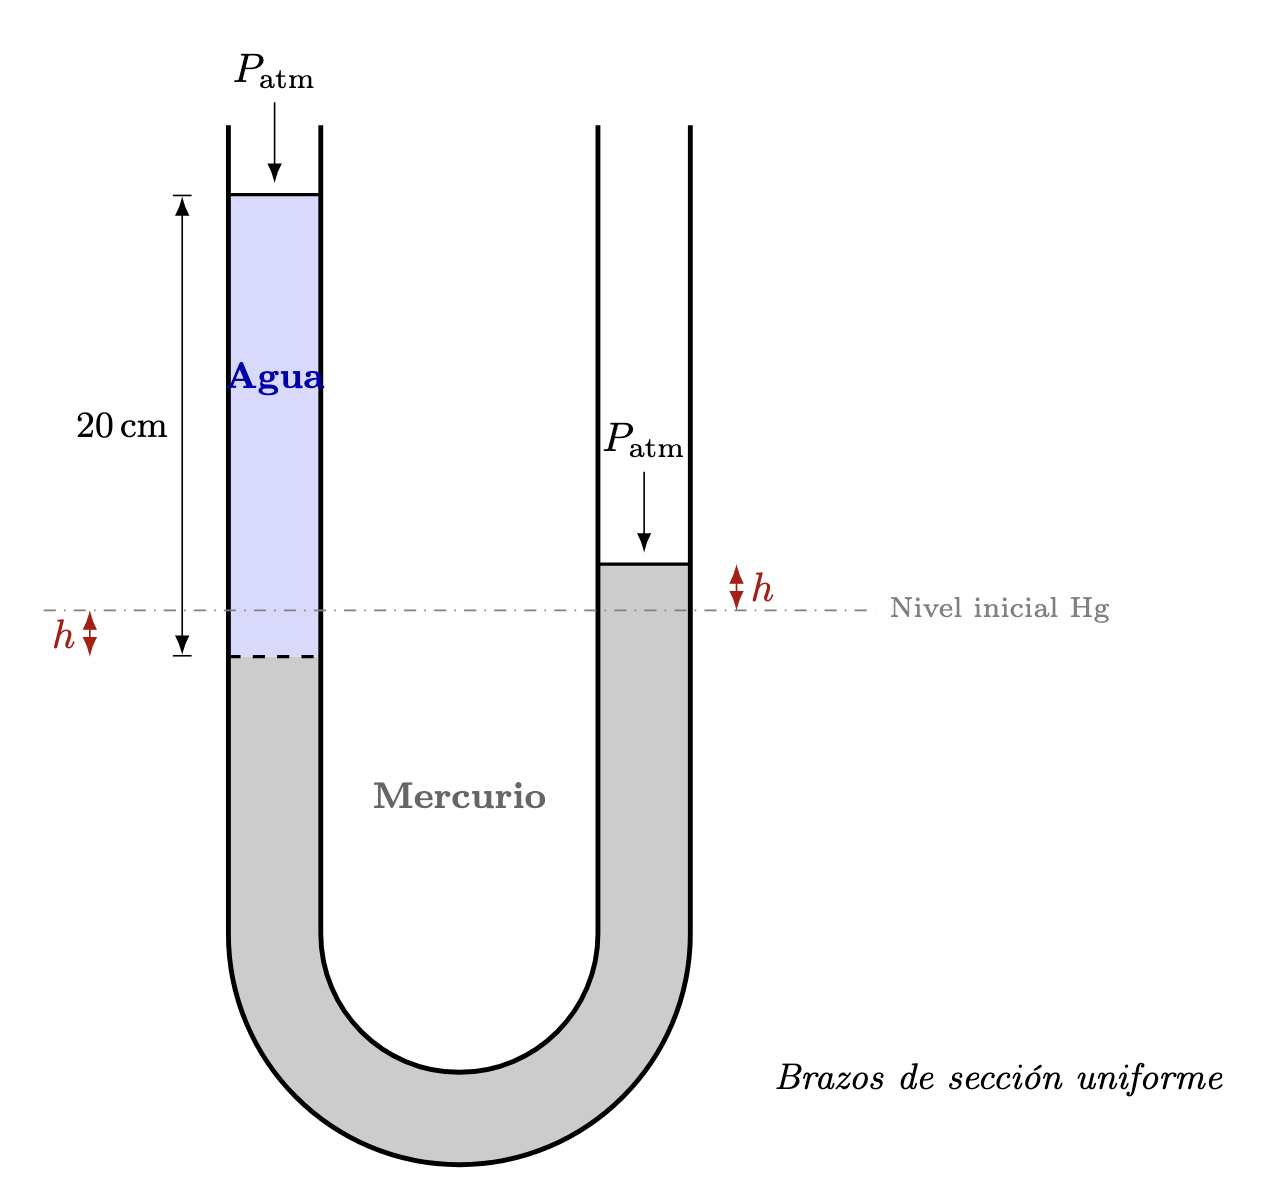
\includegraphics[keepaspectratio]{chapters/fluidos/../../images/fluidos/tubo_u.png}}

}

\caption{Esquema del tubo en U con mercurio y agua, indicando las
alturas y niveles correspondientes.}

\end{figure}%

\section*{Idea física}\label{idea-fuxedsica-1}
\addcontentsline{toc}{section}{Idea física}

\markright{Idea física}

La idea central es comparar presiones a una \textbf{misma altura dentro
del mercurio}.

Cuando se vierte agua en el brazo izquierdo, su peso adicional empuja
hacia abajo al mercurio en ese lado. Como el tubo tiene la misma sección
transversal en ambos brazos, el nivel del mercurio:

\begin{itemize}
\tightlist
\item
  \textbf{desciende} una cantidad \(x\) en el brazo izquierdo;
\item
  \textbf{asciende} una cantidad \(x\) en el brazo derecho.
\end{itemize}

Por ello, la diferencia total de niveles de mercurio entre ambos lados
es

\[
2x.
\]

El equilibrio hidrostático se obtiene al igualar:

\begin{itemize}
\tightlist
\item
  la presión producida por la columna de agua;
\item
  la presión producida por la diferencia de niveles del mercurio.
\end{itemize}

\section*{Datos}\label{datos}
\addcontentsline{toc}{section}{Datos}

\markright{Datos}

Altura de la columna de agua: \[
h=20\ \text{cm}=0.20\ \text{m}
\]

Densidad del agua: \[
\rho_{\text{agua}}=1000\ \text{kg/m}^3
\]

Densidad del mercurio: \[
\rho_{\text{Hg}}=13600\ \text{kg/m}^3
\]

\section*{Relación de equilibrio
hidrostático}\label{relaciuxf3n-de-equilibrio-hidrostuxe1tico}
\addcontentsline{toc}{section}{Relación de equilibrio hidrostático}

\markright{Relación de equilibrio hidrostático}

La presión ejercida por la columna de agua debe equilibrarse con la
presión correspondiente a la diferencia de alturas del mercurio. Así,

\[
\rho_{\text{agua}}gh=\rho_{\text{Hg}}g(2x).
\]

El factor \(g\) aparece en ambos lados, por lo que se cancela:

\[
\rho_{\text{agua}}h=\rho_{\text{Hg}}(2x).
\]

Despejando \(x\):

\[
x=\frac{\rho_{\text{agua}}h}{2\rho_{\text{Hg}}}.
\]

\section*{Sustitución numérica}\label{sustituciuxf3n-numuxe9rica}
\addcontentsline{toc}{section}{Sustitución numérica}

\markright{Sustitución numérica}

Sustituyendo los valores:

\[
x=\frac{(1000)(0.20)}{2(13600)}.
\]

Entonces,

\[
x=\frac{200}{27200}=7.35\times10^{-3}\ \text{m}.
\]

Convertimos a centímetros:

\[
x=7.35\times10^{-3}\ \text{m}=0.735\ \text{cm}.
\]

\section*{Resultado}\label{resultado}
\addcontentsline{toc}{section}{Resultado}

\markright{Resultado}

La elevación del mercurio en el brazo opuesto es

\[
\boxed{x\approx 0.74\ \text{cm}}.
\]

\section*{Interpretación física}\label{interpretaciuxf3n-fuxedsica}
\addcontentsline{toc}{section}{Interpretación física}

\markright{Interpretación física}

El valor obtenido es pequeño, lo cual tiene sentido físico. El mercurio
es mucho más denso que el agua, así que una columna relativamente grande
de agua se compensa con una variación pequeña en el nivel del mercurio.

Dicho de otro modo: como el mercurio pesa mucho más por unidad de
volumen, no necesita desplazarse demasiado para producir la diferencia
de presión necesaria.

\section*{Comentario didáctico}\label{comentario-diduxe1ctico}
\addcontentsline{toc}{section}{Comentario didáctico}

\markright{Comentario didáctico}

En este problema aparecen dos ideas importantes:

\begin{enumerate}
\def\labelenumi{\arabic{enumi}.}
\tightlist
\item
  \textbf{La presión a una misma altura, dentro de un mismo fluido
  continuo, debe ser la misma} cuando el sistema está en equilibrio.
\item
  \textbf{La conservación de volumen} en tubos con igual sección implica
  que, si en un lado el nivel baja \(x\), en el otro sube también \(x\).
\end{enumerate}

Por eso la diferencia total entre niveles no es \(x\), sino

\[
2x.
\]

Ese detalle suele ser el punto más importante del ejercicio.

\chapter{Problema 3. Sustentación de un ala por diferencia de
velocidades}\label{problema-3.-sustentaciuxf3n-de-un-ala-por-diferencia-de-velocidades}

\section{Enunciado}\label{enunciado-2}

El aire fluye horizontalmente alrededor de las alas de una avioneta. La
rapidez del aire es de \textbf{82 m/s} por la parte superior del ala y
de \textbf{68 m/s} por la parte inferior. El área total efectiva de las
alas es de \textbf{18.5 m²}. Considere una densidad del aire igual a

\[
\rho = 1.18\ \text{kg/m}^3.
\]

Determine la fuerza vertical neta ejercida por el aire sobre la
avioneta.

\section{Idea física}\label{idea-fuxedsica-2}

Este problema usa la ecuación de Bernoulli. Si la rapidez es mayor en la
parte superior, entonces la presión arriba es menor. La diferencia de
presión entre la cara inferior y la superior produce una fuerza neta
hacia arriba.

\section{Desarrollo}\label{desarrollo}

\subsection{Paso 1. Diferencia de
presión}\label{paso-1.-diferencia-de-presiuxf3n}

Aplicamos Bernoulli entre la parte superior e inferior, suponiendo la
misma altura:

\[
p_{sup}+\frac12\rho v_{sup}^2 = p_{inf}+\frac12\rho v_{inf}^2.
\]

Despejamos la diferencia de presión:

\[
p_{inf}-p_{sup} = \frac12\rho\left(v_{sup}^2-v_{inf}^2\right).
\]

Sustituyendo valores:

\[
\Delta p = \frac12(1.18)\left(82^2-68^2\right).
\]

Calculamos los cuadrados:

\[
82^2=6724,
\qquad
68^2=4624.
\]

Entonces:

\[
\Delta p = 0.59(6724-4624)=0.59(2100)=1239\ \text{Pa}.
\]

\subsection{Paso 2. Fuerza neta}\label{paso-2.-fuerza-neta}

La fuerza de sustentación idealizada vale

\[
F = \Delta p\,A.
\]

Sustituyendo:

\[
F=(1239)(18.5)=22921.5\ \text{N}.
\]

\section{Resultado}\label{resultado-1}

\[
\boxed{F\approx 2.29\times10^4\ \text{N}}
\]

La fuerza es \textbf{hacia arriba}.

\chapter{Problema 4. Umbral de cavitación en un
Venturi}\label{problema-4.-umbral-de-cavitaciuxf3n-en-un-venturi}

\section{Enunciado}\label{enunciado-3}

En un tubo de Venturi circula agua a \textbf{20 °C}. Los radios de las
secciones son

\[
r_1=10\ \text{cm}, \qquad r_2=2.0\ \text{cm}.
\]

Se sabe que el número de cavitación crítico para que comiencen a
formarse burbujas es

\[
Ca=0.40.
\]

Determine la rapidez del fluido en la sección ancha para que empiece la
cavitación en la sección angosta, suponiendo que la presión en la
sección ancha es atmosférica:

\[
p_1 = 1.013\times10^5\ \text{Pa}.
\]

Para el agua a \(20^\circ\)C, tome:

\[
\rho=998\ \text{kg/m}^3,
\qquad
p_v = 2.34\times10^3\ \text{Pa}.
\]

\section{Idea física}\label{idea-fuxedsica-3}

La cavitación empieza cuando la presión local se acerca a la presión de
vapor. El número de cavitación dado es

\[
Ca = \frac{p-p_v}{\tfrac12\rho v^2}.
\]

La región crítica será la sección angosta, donde la velocidad es mayor y
la presión es menor.

\section{Desarrollo}\label{desarrollo-1}

\subsection{Paso 1. Relación entre velocidades por
continuidad}\label{paso-1.-relaciuxf3n-entre-velocidades-por-continuidad}

Por continuidad:

\[
A_1v_1=A_2v_2.
\]

Como \(A\propto r^2\),

\[
v_2 = \frac{A_1}{A_2}v_1 = \frac{r_1^2}{r_2^2}v_1.
\]

Sustituyendo:

\[
v_2 = \frac{(10)^2}{(2)^2}v_1 = 25v_1.
\]

\subsection{Paso 2. Bernoulli entre las dos
secciones}\label{paso-2.-bernoulli-entre-las-dos-secciones}

Suponiendo igual altura:

\[
p_1 + \frac12\rho v_1^2 = p_2 + \frac12\rho v_2^2.
\]

Despejamos \(p_2\):

\[
p_2 = p_1 + \frac12\rho\left(v_1^2-v_2^2\right).
\]

Como \(v_2=25v_1\),

\[
p_2 = p_1 - \frac12\rho(624)v_1^2.
\]

\subsection{Paso 3. Usar la condición de
cavitación}\label{paso-3.-usar-la-condiciuxf3n-de-cavitaciuxf3n}

En la garganta,

\[
Ca = \frac{p_2-p_v}{\tfrac12\rho v_2^2} = 0.40.
\]

Entonces,

\[
p_2 - p_v = 0.40\left(\frac12\rho v_2^2\right).
\]

Sustituimos \(v_2=25v_1\):

\[
p_2 - p_v = 0.40\left(\frac12\rho (625v_1^2)\right)=125\rho v_1^2.
\]

Pero también

\[
p_2 = p_1 - 312\rho v_1^2.
\]

Entonces,

\[
p_1 - 312\rho v_1^2 - p_v = 125\rho v_1^2.
\]

Agrupando:

\[
p_1 - p_v = 437\rho v_1^2.
\]

Despejando \(v_1\):

\[
v_1^2 = \frac{p_1-p_v}{437\rho}.
\]

Sustituyendo:

\[
v_1^2 = \frac{1.013\times10^5 - 2.34\times10^3}{437(998)} \approx 0.2269.
\]

\[
v_1 \approx 0.476\ \text{m/s}.
\]

\section{Resultado}\label{resultado-2}

\[
\boxed{v_1\approx 0.48\ \text{m/s}},
\qquad
\boxed{v_2\approx 11.9\ \text{m/s}}.
\]

\chapter{Problema 5. Descarga por un orificio y trayectoria del
chorro}\label{problema-5.-descarga-por-un-orificio-y-trayectoria-del-chorro}

\section{Enunciado}\label{enunciado-4}

Un tanque abierto contiene agua. En una pared lateral hay un orificio
circular de \textbf{2.0 cm de diámetro}, localizado \textbf{4.0 m por
debajo} del nivel del agua.

Se pide:

\begin{enumerate}
\def\labelenumi{\alph{enumi})}
\item
  el volumen de agua que sale por minuto;
\item
  si el chorro sale inicialmente horizontal y el orificio está a
  \textbf{1.20 m} sobre el piso, determinar el alcance horizontal hasta
  tocar el piso;
\item
  decidir si el flujo al salir es laminar o turbulento, usando el número
  de Reynolds. Tome para el agua:
\end{enumerate}

\[
\mu = 1.0\times10^{-3}\ \text{Pa·s}.
\]

\section{Desarrollo}\label{desarrollo-2}

Por Torricelli,

\[
v = \sqrt{2gh}=\sqrt{2(9.81)(4.0)}=8.86\ \text{m/s}.
\]

El área del orificio es

\[
A=\pi(0.010)^2=3.1416\times10^{-4}\ \text{m}^2.
\]

Entonces el gasto es

\[
Q=Av=(3.1416\times10^{-4})(8.86)=2.783\times10^{-3}\ \text{m}^3/\text{s}.
\]

Por minuto:

\[
Q_{min}=60Q=0.167\ \text{m}^3/\text{min}=167\ \text{L/min}.
\]

Para la trayectoria horizontal, el tiempo de caída desde
\(1.20\ \text{m}\) es

\[
t=\sqrt{\frac{2(1.20)}{9.81}}=0.4946\ \text{s}.
\]

Por tanto,

\[
x=vt=(8.86)(0.4946)=4.38\ \text{m}.
\]

El número de Reynolds es

\[
Re=\frac{\rho vd}{\mu}=\frac{(1000)(8.86)(0.020)}{10^{-3}}=177200.
\]

Por ello, el flujo es turbulento.

\section{Resultado}\label{resultado-3}

\[
\boxed{Q\approx 0.167\ \text{m}^3/\text{min}=167\ \text{L/min}}
\]

\[
\boxed{x\approx 4.38\ \text{m}}
\]

\[
\boxed{\text{flujo turbulento}}
\]

\chapter{Problema 6. Tiempo de vaciado de un tanque
cilíndrico}\label{problema-6.-tiempo-de-vaciado-de-un-tanque-ciluxedndrico}

\section{Enunciado}\label{enunciado-5}

Un tanque cilíndrico grande, abierto al aire, contiene aceite de
densidad

\[
\rho = 840\ \text{kg/m}^3.
\]

El tanque tiene \textbf{radio \(R=0.60\ \text{m}\)} y contiene líquido
hasta una altura inicial

\[
H=1.80\ \text{m}.
\]

En el fondo se abre un pequeño orificio de radio

\[
r=0.012\ \text{m},
\]

con \(r\ll R\).

Se pide:

\begin{enumerate}
\def\labelenumi{\alph{enumi})}
\item
  calcular el tiempo de vaciado ignorando viscosidad;
\item
  explicar qué ocurriría si se considerara la viscosidad.
\end{enumerate}

\section{Desarrollo}\label{desarrollo-3}

Las áreas son

\[
A=\pi(0.60)^2=1.131\ \text{m}^2,
\qquad
a=\pi(0.012)^2=4.524\times10^{-4}\ \text{m}^2.
\]

Con Torricelli, el vaciado satisface

\[
A\frac{dh}{dt}=-a\sqrt{2gh}.
\]

Separando e integrando, se obtiene

\[
T = \frac{2A\sqrt{H}}{a\sqrt{2g}}.
\]

Sustituyendo:

\[
T = \frac{2(1.131)\sqrt{1.80}}{(4.524\times10^{-4})\sqrt{19.62}} \approx 1514\ \text{s}.
\]

En minutos:

\[
T\approx 25.2\ \text{min}.
\]

Si se toma en cuenta la viscosidad, la rapidez de salida disminuye y el
tiempo real de vaciado aumenta.

\section{Resultado}\label{resultado-4}

\[
\boxed{T\approx 1.51\times10^3\ \text{s}\approx 25.2\ \text{min}}
\]

\[
\boxed{\text{con viscosidad, el tanque tardaría más en vaciarse}}
\]

\chapter{Resumen final de respuestas}\label{resumen-final-de-respuestas}

\begin{enumerate}
\def\labelenumi{\arabic{enumi}.}
\tightlist
\item
  \(p_{sup}=0\ \text{Pa}\),
  \(p_{inf}\approx 1.62\times10^3\ \text{Pa}\),
  \(m\approx 1.87\ \text{kg}\),
  \(\rho_c\approx 9.19\times10^2\ \text{kg/m}^3\).
\item
  Elevación del mercurio: \(0.74\ \text{cm}\).
\item
  Fuerza de sustentación: \(2.29\times10^4\ \text{N}\) hacia arriba.
\item
  Cavitación: \(v_1\approx 0.48\ \text{m/s}\) y
  \(v_2\approx 11.9\ \text{m/s}\).
\item
  Caudal: \(167\ \text{L/min}\), alcance: \(4.38\ \text{m}\), flujo
  turbulento.
\item
  Tiempo ideal de vaciado: \(25.2\ \text{min}\).
\end{enumerate}

\part{Ondas}

\chapter{Oscilador armónico y series de
Fourier}\label{oscilador-armuxf3nico-y-series-de-fourier}

Introducción a fluidos, ondas y termodinámica

\hfill\break

\chapter{Oscilador armónico simple}\label{sec-oscilador}

El \textbf{oscilador armónico simple} (OAS) describe el movimiento de
cualquier sistema que, al desplazarse de su posición de equilibrio,
experimenta una fuerza restauradora proporcional al desplazamiento
(Halliday, Resnick, and Walker 2014, cap. 15):

\[
F = -kx
\]

donde \(k\) es la constante de resorte (N/m) y \(x\) es el
desplazamiento respecto al equilibrio. Aplicando la segunda ley de
Newton se obtiene la \textbf{ecuación diferencial del OAS}:

\[
m\ddot{x} + kx = 0
\quad \Longrightarrow \quad
\ddot{x} + \omega_0^2\, x = 0
\]

con la \textbf{frecuencia angular natural}

\[
\boxed{\omega_0 = \sqrt{\frac{k}{m}}}
\]

Para entender el OAS más allá de las fórmulas, es útil visualizarlo como
una \textbf{proyección del movimiento circular}. Imagina una partícula
girando en un círculo de radio \(A\) con velocidad angular constante
\(\omega_0\). La sombra de esa partícula proyectada sobre el diámetro
del círculo realiza exactamente un movimiento armónico simple.

\begin{Shaded}
\begin{Highlighting}[]
\ImportTok{import}\NormalTok{ numpy }\ImportTok{as}\NormalTok{ np}
\ImportTok{import}\NormalTok{ plotly.graph\_objects }\ImportTok{as}\NormalTok{ go}

\CommentTok{\# Parámetros del sistema}
\NormalTok{A }\OperatorTok{=} \FloatTok{1.0}          \CommentTok{\# Amplitud (Radio del círculo)}
\NormalTok{omega\_0 }\OperatorTok{=} \FloatTok{1.0}    \CommentTok{\# Frecuencia angular}
\NormalTok{phi }\OperatorTok{=}\NormalTok{ np.pi}\OperatorTok{/}\DecValTok{4}    \CommentTok{\# Fase inicial (45 grados)}
\NormalTok{t\_max }\OperatorTok{=} \DecValTok{10}
\NormalTok{fps }\OperatorTok{=} \DecValTok{30}
\NormalTok{t\_steps }\OperatorTok{=}\NormalTok{ np.linspace(}\DecValTok{0}\NormalTok{, t\_max, t\_max }\OperatorTok{*}\NormalTok{ fps)}

\CommentTok{\# Datos del círculo de referencia}
\NormalTok{theta\_circle }\OperatorTok{=}\NormalTok{ np.linspace(}\DecValTok{0}\NormalTok{, }\DecValTok{2}\OperatorTok{*}\NormalTok{np.pi, }\DecValTok{100}\NormalTok{)}
\NormalTok{x\_circle }\OperatorTok{=}\NormalTok{ A }\OperatorTok{*}\NormalTok{ np.cos(theta\_circle)}
\NormalTok{y\_circle }\OperatorTok{=}\NormalTok{ A }\OperatorTok{*}\NormalTok{ np.sin(theta\_circle)}

\CommentTok{\# Crear la figura}
\NormalTok{fig }\OperatorTok{=}\NormalTok{ go.Figure()}

\CommentTok{\# 1. Dibujar el círculo estático}
\NormalTok{fig.add\_trace(go.Scatter(x}\OperatorTok{=}\NormalTok{x\_circle, y}\OperatorTok{=}\NormalTok{y\_circle, mode}\OperatorTok{=}\StringTok{\textquotesingle{}lines\textquotesingle{}}\NormalTok{, }
\NormalTok{                         line}\OperatorTok{=}\BuiltInTok{dict}\NormalTok{(color}\OperatorTok{=}\StringTok{\textquotesingle{}lightgray\textquotesingle{}}\NormalTok{, dash}\OperatorTok{=}\StringTok{\textquotesingle{}dash\textquotesingle{}}\NormalTok{),}
\NormalTok{                         name}\OperatorTok{=}\StringTok{\textquotesingle{}Trayectoria Circular\textquotesingle{}}\NormalTok{))}

\CommentTok{\# 2. Línea de proyección (diámetro horizontal)}
\NormalTok{fig.add\_trace(go.Scatter(x}\OperatorTok{=}\NormalTok{[}\OperatorTok{{-}}\NormalTok{A, A], y}\OperatorTok{=}\NormalTok{[}\DecValTok{0}\NormalTok{, }\DecValTok{0}\NormalTok{], mode}\OperatorTok{=}\StringTok{\textquotesingle{}lines\textquotesingle{}}\NormalTok{, }
\NormalTok{                         line}\OperatorTok{=}\BuiltInTok{dict}\NormalTok{(color}\OperatorTok{=}\StringTok{\textquotesingle{}black\textquotesingle{}}\NormalTok{, width}\OperatorTok{=}\DecValTok{1}\NormalTok{),}
\NormalTok{                         showlegend}\OperatorTok{=}\VariableTok{False}\NormalTok{))}

\CommentTok{\# 3. Punto en movimiento circular (La Partícula)}
\NormalTok{fig.add\_trace(go.Scatter(x}\OperatorTok{=}\NormalTok{[A}\OperatorTok{*}\NormalTok{np.cos(phi)], y}\OperatorTok{=}\NormalTok{[A}\OperatorTok{*}\NormalTok{np.sin(phi)], }
\NormalTok{                         mode}\OperatorTok{=}\StringTok{\textquotesingle{}markers+lines\textquotesingle{}}\NormalTok{, name}\OperatorTok{=}\StringTok{\textquotesingle{}Partícula (MCU)\textquotesingle{}}\NormalTok{,}
\NormalTok{                         marker}\OperatorTok{=}\BuiltInTok{dict}\NormalTok{(color}\OperatorTok{=}\StringTok{\textquotesingle{}blue\textquotesingle{}}\NormalTok{, size}\OperatorTok{=}\DecValTok{10}\NormalTok{)))}

\CommentTok{\# 4. Sombra/Proyección (El OAS)}
\NormalTok{fig.add\_trace(go.Scatter(x}\OperatorTok{=}\NormalTok{[A}\OperatorTok{*}\NormalTok{np.cos(phi)], y}\OperatorTok{=}\NormalTok{[}\DecValTok{0}\NormalTok{], }
\NormalTok{                         mode}\OperatorTok{=}\StringTok{\textquotesingle{}markers\textquotesingle{}}\NormalTok{, name}\OperatorTok{=}\StringTok{\textquotesingle{}Sombra (OAS)\textquotesingle{}}\NormalTok{,}
\NormalTok{                         marker}\OperatorTok{=}\BuiltInTok{dict}\NormalTok{(color}\OperatorTok{=}\StringTok{\textquotesingle{}red\textquotesingle{}}\NormalTok{, size}\OperatorTok{=}\DecValTok{12}\NormalTok{, symbol}\OperatorTok{=}\StringTok{\textquotesingle{}square\textquotesingle{}}\NormalTok{)))}

\CommentTok{\# Configuración de la animación}
\NormalTok{frames }\OperatorTok{=}\NormalTok{ []}
\ControlFlowTok{for}\NormalTok{ t }\KeywordTok{in}\NormalTok{ t\_steps:}
\NormalTok{    current\_angle }\OperatorTok{=}\NormalTok{ omega\_0 }\OperatorTok{*}\NormalTok{ t }\OperatorTok{+}\NormalTok{ phi}
\NormalTok{    curr\_x }\OperatorTok{=}\NormalTok{ A }\OperatorTok{*}\NormalTok{ np.cos(current\_angle)}
\NormalTok{    curr\_y }\OperatorTok{=}\NormalTok{ A }\OperatorTok{*}\NormalTok{ np.sin(current\_angle)}
    
\NormalTok{    frames.append(go.Frame(data}\OperatorTok{=}\NormalTok{[}
\NormalTok{        go.Scatter(x}\OperatorTok{=}\NormalTok{[curr\_x], y}\OperatorTok{=}\NormalTok{[curr\_y]), }\CommentTok{\# Punto azul}
\NormalTok{        go.Scatter(x}\OperatorTok{=}\NormalTok{[curr\_x], y}\OperatorTok{=}\NormalTok{[}\DecValTok{0}\NormalTok{])       }\CommentTok{\# Punto rojo (proyección)}
\NormalTok{    ], traces}\OperatorTok{=}\NormalTok{[}\DecValTok{2}\NormalTok{, }\DecValTok{3}\NormalTok{]))}

\NormalTok{fig.frames }\OperatorTok{=}\NormalTok{ frames}

\CommentTok{\# Diseño y Controles}
\NormalTok{fig.update\_layout(}
\NormalTok{    title}\OperatorTok{=}\StringTok{"OAS como proyección del Movimiento Circular"}\NormalTok{,}
\NormalTok{    xaxis}\OperatorTok{=}\BuiltInTok{dict}\NormalTok{(}\BuiltInTok{range}\OperatorTok{=}\NormalTok{[}\OperatorTok{{-}}\FloatTok{1.5}\NormalTok{, }\FloatTok{1.5}\NormalTok{], autorange}\OperatorTok{=}\VariableTok{False}\NormalTok{, zeroline}\OperatorTok{=}\VariableTok{False}\NormalTok{),}
\NormalTok{    yaxis}\OperatorTok{=}\BuiltInTok{dict}\NormalTok{(}\BuiltInTok{range}\OperatorTok{=}\NormalTok{[}\OperatorTok{{-}}\FloatTok{1.5}\NormalTok{, }\FloatTok{1.5}\NormalTok{], autorange}\OperatorTok{=}\VariableTok{False}\NormalTok{, zeroline}\OperatorTok{=}\VariableTok{False}\NormalTok{),}
\NormalTok{    template}\OperatorTok{=}\StringTok{"plotly\_white"}\NormalTok{,}
\NormalTok{    updatemenus}\OperatorTok{=}\NormalTok{[}\BuiltInTok{dict}\NormalTok{(}\BuiltInTok{type}\OperatorTok{=}\StringTok{"buttons"}\NormalTok{, buttons}\OperatorTok{=}\NormalTok{[}\BuiltInTok{dict}\NormalTok{(label}\OperatorTok{=}\StringTok{"Reproducir"}\NormalTok{, method}\OperatorTok{=}\StringTok{"animate"}\NormalTok{, }
\NormalTok{                                                    args}\OperatorTok{=}\NormalTok{[}\VariableTok{None}\NormalTok{, \{}\StringTok{"frame"}\NormalTok{: \{}\StringTok{"duration"}\NormalTok{: }\DecValTok{33}\NormalTok{, }\StringTok{"redraw"}\NormalTok{: }\VariableTok{False}\NormalTok{\}\}])])]}
\NormalTok{)}

\NormalTok{fig.show()}
\end{Highlighting}
\end{Shaded}

\begin{verbatim}
Unable to display output for mime type(s): text/html
\end{verbatim}

\begin{verbatim}
Unable to display output for mime type(s): text/html
\end{verbatim}

\begin{itemize}
\tightlist
\item
  \textbf{¿Por qué \(\omega_0\) depende de \(k\) y \(m\)?}:
  Intuitivamente, una \(k\) grande significa un resorte ``duro'' que
  recupera su forma con fuerza, acelerando la masa rápidamente (mayor
  frecuencia). Una \(m\) grande aporta más inercia, haciendo que el
  sistema sea más ``pesado'' para cambiar de dirección (menor
  frecuencia).
\item
  \textbf{La Fase (\(\varphi\))}: Representa el ``estado'' del
  cronómetro al iniciar el estudio. Nos indica en qué punto del ciclo de
  oscilación empezamos a contar el tiempo.
\end{itemize}

\subsection{Solución general}\label{soluciuxf3n-general}

La solución general es una combinación de seno y coseno (Giancoli 2008,
cap. 14):

\[
x(t) = A\cos(\omega_0 t + \varphi)
\]

donde \(A\) es la \textbf{amplitud} (determinada por condiciones
iniciales) y \(\varphi\) es la \textbf{fase inicial}. Las relaciones
clave son:

\begin{longtable}[]{@{}lll@{}}
\toprule\noalign{}
Cantidad & Expresión & Unidades \\
\midrule\noalign{}
\endhead
\bottomrule\noalign{}
\endlastfoot
\textbf{Frecuencia angular} & \(\omega_0 = \sqrt{k/m}\) & rad/s \\
\textbf{Periodo} & \(T = 2\pi/\omega_0\) & s \\
\textbf{Frecuencia} & \(f = 1/T\) & Hz \\
\textbf{Velocidad máxima} & \(v_\text{máx} = A\omega_0\) & m/s \\
\textbf{Aceleración máxima} & \(a_\text{máx} = A\omega_0^2\) & m/s² \\
\end{longtable}

\subsection{Energía del oscilador}\label{energuxeda-del-oscilador}

La energía mecánica total se \textbf{conserva} a lo largo del movimiento
(Halliday, Resnick, and Walker 2014, secs. 15--4):

\[
E = \underbrace{\frac{1}{2}mv^2}_{E_\text{cinética}} +
    \underbrace{\frac{1}{2}kx^2}_{E_\text{potencial}} =
    \frac{1}{2}kA^2 = \text{constante}
\]

En la posición de equilibrio (\(x=0\)) toda la energía es cinética; en
los extremos (\(x = \pm A\)) toda es potencial.

\section{Conexión con Series de Fourier}\label{sec-fourier-link}

En la práctica, los sistemas físicos reales suelen estar sujetos a
fuerzas externas periódicas que no son puramente sinusoidales. Aquí es
donde las \textbf{Series de Fourier} permiten expandir el análisis del
OAS.

Cualquier fuerza periódica \(F(t)\) (como una onda cuadrada o una
vibración mecánica compleja) puede descomponerse en una suma de
armónicos simples:

\[F(t) = \frac{a_0}{2} + \sum_{n=1}^{\infty} [a_n \cos(n\omega t) + b_n \sin(n\omega t)]\]

\subsection{¿Por qué es fundamental para el estudio del
oscilador?}\label{por-quuxe9-es-fundamental-para-el-estudio-del-oscilador}

\begin{enumerate}
\def\labelenumi{\arabic{enumi}.}
\tightlist
\item
  \textbf{Principio de Superposición}: Gracias a que la ecuación del OAS
  es lineal, la respuesta total del sistema es simplemente la suma de
  las respuestas individuales a cada armónico de la fuerza externa.
\item
  \textbf{Resonancia Selectiva}: Un oscilador con frecuencia natural
  \(\omega_0\) ``filtrará'' la fuerza externa. Si uno de los componentes
  de la serie de Fourier de la fuerza (\(n\omega\)) está cerca de
  \(\omega_0\), ese término dominará el movimiento, provocando grandes
  amplitudes.
\end{enumerate}

\begin{quote}
\textbf{Ejemplo visual}: En el caso de una \textbf{onda cuadrada} (ver
Ejercicio 2 de la tarea), aunque la fuerza parece constante a trozos, el
oscilador ``siente'' los armónicos impares (\(1, 3, 5 \dots\)). Si la
frecuencia natural del oscilador coincide con el tercer armónico,
veremos una oscilación dominante a esa frecuencia.
\end{quote}

\section{Ejercicios --- Bloque 1: Oscilador
armónico}\label{ejercicios-bloque-1-oscilador-armuxf3nico}

\subsection*{Ejercicio 1 · Identificar
parámetros}\label{ejercicio-1-identificar-paruxe1metros}
\addcontentsline{toc}{subsection}{Ejercicio 1 · Identificar parámetros}

\begin{quote}
\textbf{Nivel:} ⬤○○ básico
\end{quote}

Un resorte tiene constante \(k = 50\,\text{N/m}\). Se cuelga una masa de
\(m = 200\,\text{g}\) y se le da un desplazamiento inicial de
\(x_0 = 5\,\text{cm}\) soltándola desde el reposo.

\begin{enumerate}
\def\labelenumi{\alph{enumi})}
\tightlist
\item
  Calcula la frecuencia angular \(\omega_0\).
\item
  Calcula el periodo \(T\) y la frecuencia \(f\).
\item
  Escribe la ecuación de movimiento \(x(t)\).
\end{enumerate}

\begin{tcolorbox}[enhanced jigsaw, breakable, arc=.35mm, opacitybacktitle=0.6, opacityback=0, rightrule=.15mm, leftrule=.75mm, toptitle=1mm, colback=white, toprule=.15mm, colbacktitle=quarto-callout-tip-color!10!white, bottomrule=.15mm, bottomtitle=1mm, titlerule=0mm, title=\textcolor{quarto-callout-tip-color}{\faLightbulb}\hspace{0.5em}{Pista}, coltitle=black, colframe=quarto-callout-tip-color-frame, left=2mm]

Recuerda convertir unidades antes de sustituir:
\(m = 0.200\,\text{kg}\), \(x_0 = 0.05\,\text{m}\). Como la velocidad
inicial es cero, \(\varphi = 0\) y la amplitud es \(A = x_0\).

\end{tcolorbox}

\subsection*{Ejercicio 2 · Energía en el
oscilador}\label{ejercicio-2-energuxeda-en-el-oscilador}
\addcontentsline{toc}{subsection}{Ejercicio 2 · Energía en el oscilador}

\begin{quote}
\textbf{Nivel:} ⬤○○ básico
\end{quote}

Usando los resultados del Ejercicio 1:

\begin{enumerate}
\def\labelenumi{\alph{enumi})}
\tightlist
\item
  Calcula la energía mecánica total \(E\).
\item
  Calcula la velocidad máxima \(v_\text{máx}\).
\item
  ¿En qué posición \(x^*\) la energía cinética es igual a la energía
  potencial?
\end{enumerate}

\begin{tcolorbox}[enhanced jigsaw, breakable, arc=.35mm, opacitybacktitle=0.6, opacityback=0, rightrule=.15mm, leftrule=.75mm, toptitle=1mm, colback=white, toprule=.15mm, colbacktitle=quarto-callout-tip-color!10!white, bottomrule=.15mm, bottomtitle=1mm, titlerule=0mm, title=\textcolor{quarto-callout-tip-color}{\faLightbulb}\hspace{0.5em}{Pista}, coltitle=black, colframe=quarto-callout-tip-color-frame, left=2mm]

Para el inciso (c) plantea \(\frac{1}{2}mv^2 = \frac{1}{2}kx^2\) y
recuerda que \(v^2 = \omega_0^2(A^2 - x^2)\) (se obtiene de la
conservación de energía).

\end{tcolorbox}

\subsection*{Ejercicio 3 · Lectura e interpretación de
gráfica}\label{ejercicio-3-lectura-e-interpretaciuxf3n-de-gruxe1fica}
\addcontentsline{toc}{subsection}{Ejercicio 3 · Lectura e interpretación
de gráfica}

\begin{quote}
\textbf{Nivel:} ⬤⬤○ intermedio
\end{quote}

La posición de un oscilador está dada por:

\[
x(t) = 3\cos\!\left(\frac{2\pi}{0.8}\,t\right)\,\text{cm}
\]

\begin{enumerate}
\def\labelenumi{\alph{enumi})}
\tightlist
\item
  Identifica la amplitud, el periodo y la frecuencia.
\item
  Evalúa \(x(0.2\,\text{s})\) y \(x(0.4\,\text{s})\).
\item
  Bosqueja la gráfica \(x\) vs \(t\) para dos periodos completos. Indica
  claramente los valores en los ejes.
\end{enumerate}

\begin{tcolorbox}[enhanced jigsaw, breakable, arc=.35mm, opacitybacktitle=0.6, opacityback=0, rightrule=.15mm, leftrule=.75mm, toptitle=1mm, colback=white, toprule=.15mm, colbacktitle=quarto-callout-tip-color!10!white, bottomrule=.15mm, bottomtitle=1mm, titlerule=0mm, title=\textcolor{quarto-callout-tip-color}{\faLightbulb}\hspace{0.5em}{Pista}, coltitle=black, colframe=quarto-callout-tip-color-frame, left=2mm]

Compara con la forma general \(x(t) = A\cos(\omega t + \varphi)\). Aquí
\(\omega = 2\pi/T\), así que \(T\) se puede leer directamente del
denominador.

\end{tcolorbox}

\chapter{Series de Fourier}\label{sec-fourier}

\section{Motivación física}\label{motivaciuxf3n-fuxedsica}

Muchas señales en física --- sonido, luz, señales eléctricas, fuerzas
periódicas --- no son sinusoidales puras, pero \textbf{sí son
periódicas}. Jean-Baptiste Joseph Fourier demostró que toda función
periódica ``razonablemente bien portada'' puede escribirse como suma
(posiblemente infinita) de senos y cosenos (Kreyszig 2011, cap. 11).

\begin{quote}
\emph{``Toda función periódica es una superposición de osciladores
armónicos.''}
\end{quote}

\section{Definición de la serie}\label{definiciuxf3n-de-la-serie}

Sea \(f(x)\) una función de periodo \(2\pi\). Su \textbf{desarrollo en
serie de Fourier} es (Arfken, Weber, and Harris 2013, sec. 14.1):

\[
f(x) = \frac{a_0}{2} + \sum_{n=1}^{\infty}\bigl[a_n\cos(nx) + b_n\sin(nx)\bigr]
\]

Los coeficientes se obtienen por \textbf{ortogonalidad} de senos y
cosenos:

\[
a_0 = \frac{1}{\pi}\int_{-\pi}^{\pi} f(x)\,dx
\]

\[
a_n = \frac{1}{\pi}\int_{-\pi}^{\pi} f(x)\cos(nx)\,dx, \qquad n = 1,2,3,\ldots
\]

\[
b_n = \frac{1}{\pi}\int_{-\pi}^{\pi} f(x)\sin(nx)\,dx, \qquad n = 1,2,3,\ldots
\]

\section{Simetrías que simplifican el
cálculo}\label{simetruxedas-que-simplifican-el-cuxe1lculo}

Antes de integrar, vale la pena inspeccionar la simetría de \(f(x)\):

Simetría \textbar{} Condición \textbar{} Consecuencia \textbar{}

\textbar\textbar\textbar\textbar{} \textbar{} Función \textbf{par}
\textbar{} \(f(-x) = f(x)\) \textbar{} Todos los \(b_n = 0\) \textbar{}
\textbar{} Función \textbf{impar} \textbar{} \(f(-x) = -f(x)\)
\textbar{} \(a_0 = 0\) y todos los \(a_n = 0\) \textbar{}

Esto puede reducir el trabajo a la mitad (o más).

\section{Convergencia: teorema de
Dirichlet}\label{convergencia-teorema-de-dirichlet}

Si \(f(x)\) es periódica, acotada y tiene un número finito de
discontinuidades y extremos en un periodo, la serie de Fourier converge
(Kreyszig 2011, sec. 11.1):

\begin{itemize}
\tightlist
\item
  A \(f(x)\) en los puntos de continuidad.
\item
  Al \textbf{promedio} \(\tfrac{1}{2}[f(x^+) + f(x^-)]\) en los puntos
  de discontinuidad.
\end{itemize}

\section{Ejercicios --- Bloque 2: Series de
Fourier}\label{ejercicios-bloque-2-series-de-fourier}

\subsection*{Ejercicio 4 · Reconocer componentes de
Fourier}\label{ejercicio-4-reconocer-componentes-de-fourier}
\addcontentsline{toc}{subsection}{Ejercicio 4 · Reconocer componentes de
Fourier}

\begin{quote}
\textbf{Nivel:} ⬤○○ básico
\end{quote}

Considera la función periódica de periodo \(2\pi\) definida en
\(-\pi \le x < \pi\):

\[
f(x) = 3\sin(x) + \sin(3x)
\]

\begin{enumerate}
\def\labelenumi{\alph{enumi})}
\tightlist
\item
  ¿Esta función ya está expresada como serie de Fourier? Justifica tu
  respuesta.
\item
  Identifica los coeficientes \(b_1\), \(b_3\), y los demás \(a_n\),
  \(b_n\).
\item
  ¿Es \(f(x)\) par, impar, o ninguna? ¿Cómo se relaciona con los
  coeficientes que encontraste?
\end{enumerate}

\begin{tcolorbox}[enhanced jigsaw, breakable, arc=.35mm, opacitybacktitle=0.6, opacityback=0, rightrule=.15mm, leftrule=.75mm, toptitle=1mm, colback=white, toprule=.15mm, colbacktitle=quarto-callout-tip-color!10!white, bottomrule=.15mm, bottomtitle=1mm, titlerule=0mm, title=\textcolor{quarto-callout-tip-color}{\faLightbulb}\hspace{0.5em}{Pista}, coltitle=black, colframe=quarto-callout-tip-color-frame, left=2mm]

Una serie de Fourier es una suma de senos y cosenos con coeficientes
constantes. Si la función ya tiene esa forma, los coeficientes se leen
directamente. Recuerda que \(f(-x) = -f(x)\) caracteriza a una función
impar.

\end{tcolorbox}

\subsection*{\texorpdfstring{Ejercicio 5 · Serie de Fourier de
\(f(x) = x^2\)}{Ejercicio 5 · Serie de Fourier de f(x) = x\^{}2}}\label{ejercicio-5-serie-de-fourier-de-fx-x2}
\addcontentsline{toc}{subsection}{Ejercicio 5 · Serie de Fourier de
\(f(x) = x^2\)}

\begin{quote}
\textbf{Nivel:} ⬤⬤○ intermedio
\end{quote}

Encuentra la serie de Fourier de la función periódica de periodo
\(2\pi\) definida por:

\[
f(x) = x^2, \qquad -\pi \le x \le \pi
\]

\begin{enumerate}
\def\labelenumi{\alph{enumi})}
\tightlist
\item
  Argumenta por simetría: ¿habrá términos \(b_n\)? ¿Por qué?
\item
  Calcula \(a_0\) directamente.
\item
  Calcula \(a_n\) para \(n \ge 1\). (Necesitarás integrar por partes dos
  veces.)
\item
  Escribe la serie completa.
\item
  Evaluando en \(x = \pi\), deduce el valor de la suma: \[
  \sum_{n=1}^{\infty} \frac{1}{n^2}
  \]
\end{enumerate}

\begin{tcolorbox}[enhanced jigsaw, breakable, arc=.35mm, opacitybacktitle=0.6, opacityback=0, rightrule=.15mm, leftrule=.75mm, toptitle=1mm, colback=white, toprule=.15mm, colbacktitle=quarto-callout-tip-color!10!white, bottomrule=.15mm, bottomtitle=1mm, titlerule=0mm, title=\textcolor{quarto-callout-tip-color}{\faLightbulb}\hspace{0.5em}{Pista}, coltitle=black, colframe=quarto-callout-tip-color-frame, left=2mm]

\(x^2\) es función par → todos los \(b_n = 0\).

Para \(a_n\), la integral de tablas útil es: \[
\int x^2 \cos(nx)\,dx = \frac{2x\cos(nx)}{n^2} + \left(\frac{x^2}{n} - \frac{2}{n^3}\right)\sin(nx) + C
\]

Al evaluar en \(x = \pi\) recuerda que \(\cos(n\pi) = (-1)^n\) y la
serie converge a \(f(\pi) = \pi^2\).

\end{tcolorbox}

\subsection*{Ejercicio 6 · Onda
cuadrada}\label{ejercicio-6-onda-cuadrada}
\addcontentsline{toc}{subsection}{Ejercicio 6 · Onda cuadrada}

\begin{quote}
\textbf{Nivel:} ⬤⬤⬤ avanzado
\end{quote}

Se tiene la onda cuadrada de periodo \(2\pi\):

\[
f(x) = \begin{cases} +1 & \text{si } 0 < x < \pi \\ -1 & \text{si } -\pi < x < 0 \end{cases}
\]

\begin{enumerate}
\def\labelenumi{\alph{enumi})}
\tightlist
\item
  Antes de calcular: ¿es \(f(x)\) par o impar? ¿Habrá términos \(a_n\)?
\item
  Calcula los coeficientes \(b_n\).
\item
  Escribe la serie completa.
\item
  Evalúa el valor que predice la serie en \(x = 0\) (punto de
  discontinuidad). ¿Es consistente con el teorema de Dirichlet?
\end{enumerate}

\begin{tcolorbox}[enhanced jigsaw, breakable, arc=.35mm, opacitybacktitle=0.6, opacityback=0, rightrule=.15mm, leftrule=.75mm, toptitle=1mm, colback=white, toprule=.15mm, colbacktitle=quarto-callout-tip-color!10!white, bottomrule=.15mm, bottomtitle=1mm, titlerule=0mm, title=\textcolor{quarto-callout-tip-color}{\faLightbulb}\hspace{0.5em}{Pista}, coltitle=black, colframe=quarto-callout-tip-color-frame, left=2mm]

La onda cuadrada es función impar → \(a_0 = 0\) y \(a_n = 0\) para todo
\(n\).

Al calcular \(b_n\) notarás que los términos con \(n\) par se anulan. El
resultado esperado es: \[
f(x) = \frac{4}{\pi}\left[\sin(x) + \frac{\sin(3x)}{3} + \frac{\sin(5x)}{5} + \cdots\right]
\]

\end{tcolorbox}

\chapter{Conexión: oscilador forzado y análisis de
Fourier}\label{sec-conexion}

\section{¿Por qué importa Fourier en un
oscilador?}\label{por-quuxe9-importa-fourier-en-un-oscilador}

Cuando un oscilador armónico recibe una \textbf{fuerza periódica}
\(F(t)\), la ecuación de movimiento se vuelve:

\[
m\ddot{x} + kx = F(t)
\]

Si \(F(t)\) no es sinusoidal (por ejemplo, una onda cuadrada), el truco
es \textbf{descomponerla en serie de Fourier} (Halliday, Resnick, and
Walker 2014, secs. 15--7):

\[
F(t) = \sum_{n} F_n \sin(n\omega t)
\]

Por la \textbf{linealidad} de la ecuación diferencial, podemos resolver
por separado para cada componente \(F_n\) y sumar las respuestas. Esto
convierte un problema difícil en muchos problemas fáciles.

\subsection{Resonancia}\label{resonancia}

Cuando la frecuencia de algún armónico de la fuerza coincide con
\(\omega_0\), el sistema entra en \textbf{resonancia}: la amplitud crece
drásticamente (Giancoli 2008, secs. 14--7). Este fenómeno explica desde
la ruptura de puentes hasta el diseño de instrumentos musicales.

\section{Ejercicios --- Bloque 3:
Conexión}\label{ejercicios-bloque-3-conexiuxf3n}

\subsection*{Ejercicio 7 · Oscilador forzado con onda
cuadrada}\label{ejercicio-7-oscilador-forzado-con-onda-cuadrada}
\addcontentsline{toc}{subsection}{Ejercicio 7 · Oscilador forzado con
onda cuadrada}

\begin{quote}
\textbf{Nivel:} ⬤⬤○ intermedio --- conceptual
\end{quote}

Un oscilador tiene frecuencia natural \(\omega_0 = 3\,\text{rad/s}\). Se
le aplica la fuerza periódica del Ejercicio 6 con frecuencia fundamental
\(\omega = 1\,\text{rad/s}\).

\begin{enumerate}
\def\labelenumi{\alph{enumi})}
\tightlist
\item
  Usando la serie de Fourier de la onda cuadrada, lista las frecuencias
  presentes en la fuerza.
\item
  ¿Alguna frecuencia está cerca de \(\omega_0 = 3\,\text{rad/s}\)? ¿Qué
  fenómeno esperarías?
\item
  Si en cambio \(\omega_0 = 1\,\text{rad/s}\), ¿qué pasaría con el
  primer armónico? Describe cualitativamente.
\item
  Argumenta en tus propias palabras: ¿por qué es útil el análisis de
  Fourier para este tipo de problemas?
\end{enumerate}

\begin{tcolorbox}[enhanced jigsaw, breakable, arc=.35mm, opacitybacktitle=0.6, opacityback=0, rightrule=.15mm, leftrule=.75mm, toptitle=1mm, colback=white, toprule=.15mm, colbacktitle=quarto-callout-tip-color!10!white, bottomrule=.15mm, bottomtitle=1mm, titlerule=0mm, title=\textcolor{quarto-callout-tip-color}{\faLightbulb}\hspace{0.5em}{Pista}, coltitle=black, colframe=quarto-callout-tip-color-frame, left=2mm]

Los armónicos de la onda cuadrada son
\(\omega, 3\omega, 5\omega, \ldots\) Compara cada uno con \(\omega_0\).
Cuando \(n\omega \approx \omega_0\) hay resonancia.

\end{tcolorbox}

\subsection*{\texorpdfstring{Ejercicio 8 · Identidad de Parseval y la
suma
\(\sum 1/n^4\)}{Ejercicio 8 · Identidad de Parseval y la suma \textbackslash sum 1/n\^{}4}}\label{ejercicio-8-identidad-de-parseval-y-la-suma-sum-1n4}
\addcontentsline{toc}{subsection}{Ejercicio 8 · Identidad de Parseval y
la suma \(\sum 1/n^4\)}

\begin{quote}
\textbf{Nivel:} ⬤⬤⬤ avanzado
\end{quote}

La \textbf{identidad de Parseval} establece que la ``energía'' de una
señal se distribuye entre sus armónicos (Arfken, Weber, and Harris 2013,
sec. 14.5):

\[
\frac{1}{\pi}\int_{-\pi}^{\pi} [f(x)]^2\,dx =
\frac{a_0^2}{2} + \sum_{n=1}^{\infty}(a_n^2 + b_n^2)
\]

Usando los resultados del Ejercicio 5 (\(f(x) = x^2\)):

\begin{enumerate}
\def\labelenumi{\alph{enumi})}
\tightlist
\item
  Calcula el lado izquierdo: evalúa
  \(\dfrac{1}{\pi}\displaystyle\int_{-\pi}^{\pi} x^4\,dx\).
\item
  Sustituye los coeficientes \(a_0\) y \(a_n\) que obtuviste en el
  Ejercicio 5.
\item
  Despeja y obtén el valor de la suma: \[
  \sum_{n=1}^{\infty} \frac{1}{n^4}
  \]
\item
  Compara la estrategia usada aquí (Parseval) con la del Ejercicio 5
  (evaluar en un punto). ¿Cuál es más directa para obtener
  \(\sum 1/n^2\)? ¿Y para \(\sum 1/n^4\)?
\end{enumerate}

\begin{tcolorbox}[enhanced jigsaw, breakable, arc=.35mm, opacitybacktitle=0.6, opacityback=0, rightrule=.15mm, leftrule=.75mm, toptitle=1mm, colback=white, toprule=.15mm, colbacktitle=quarto-callout-tip-color!10!white, bottomrule=.15mm, bottomtitle=1mm, titlerule=0mm, title=\textcolor{quarto-callout-tip-color}{\faLightbulb}\hspace{0.5em}{Pista}, coltitle=black, colframe=quarto-callout-tip-color-frame, left=2mm]

El lado izquierdo es
\(\dfrac{1}{\pi}\cdot\dfrac{2\pi^5}{5} = \dfrac{2\pi^4}{5}\).

Después de sustituir \(a_n = \dfrac{4(-1)^n}{n^2}\), la suma del lado
derecho quedará expresada en términos de \(\sum 1/n^4\).

\end{tcolorbox}

\chapter{Ejemplos resueltos --- Oscilador
armónico}\label{sec-osc-resueltos}

Los siguientes ejemplos cubren el oscilador armónico desde sus
parámetros básicos hasta la resonancia, con visualizaciones interactivas
para facilitar la comprensión física de las ecuaciones.

\section{Ejemplo 1 · Movimiento libre: posición, velocidad y
aceleración}\label{sec-osc-1}

\subsection{Planteamiento}\label{planteamiento}

Un resorte horizontal de constante \(k = 8\,\text{N/m}\) tiene una masa
de \(m = 0.5\,\text{kg}\) unida a su extremo. Se desplaza la masa
\(A = 10\,\text{cm}\) de la posición de equilibrio y se suelta desde el
reposo.

\subsection{Paso 1 --- Frecuencia angular y
periodo}\label{paso-1-frecuencia-angular-y-periodo}

La frecuencia natural depende intrínsecamente de la rigidez (\(k\)) y la
inercia (\(m\)) del sistema:

\[
\omega_0 = \sqrt{\frac{k}{m}} = \sqrt{\frac{8}{0.5}} = \sqrt{16} = 4\,\text{rad/s}
\]

\[
T = \frac{2\pi}{\omega_0} = \frac{2\pi}{4} = \frac{\pi}{2} \approx 1.571\,\text{s}, \qquad
f = \frac{1}{T} \approx 0.637\,\text{Hz}
\]

\subsection{Paso 2 --- Condiciones iniciales y ecuación de
movimiento}\label{paso-2-condiciones-iniciales-y-ecuaciuxf3n-de-movimiento}

La solución general para la ecuación diferencial
\(\ddot{x} + \omega_0^2 x = 0\) es de la forma:
\[x(t) = A\cos(\omega_0 t + \varphi)\]

Para determinar la amplitud (\(A\)) y la fase inicial (\(\varphi\)),
aplicamos las condiciones impuestas por el problema:

\begin{enumerate}
\def\labelenumi{\arabic{enumi}.}
\item
  \textbf{Condición de Velocidad (Reposo):} Sabemos que
  \(\dot{x}(0) = 0\). La función velocidad es
  \(v(t) = -A\omega_0\sin(\omega_0 t + \varphi)\). Evaluando en \(t=0\):
  \[0 = -A\omega_0\sin(0 + \varphi) \implies \sin(\varphi) = 0 \implies \mathbf{\varphi = 0}\]
  Esto nos indica que la solución es un \textbf{coseno puro}, ya que el
  sistema inicia su movimiento en un punto de retorno donde la velocidad
  es nula.
\item
  \textbf{Condición de Posición (Desplazamiento):} Sabemos que
  \(x(0) = 0.1\,\text{m}\). Usando nuestra \(\varphi = 0\):
  \[0.1 = A\cos(4 \cdot 0 + 0) \implies 0.1 = A(1) \implies \mathbf{A = 0.1\,\text{m}}\]
\end{enumerate}

\textbf{Ecuación final de movimiento:} \[x(t) = 0.1\cos(4t)\,\text{m}\]

Derivando sucesivamente obtenemos la cinemática completa:

\[
v(t) = \dot{x}(t) = -A\omega_0\sin(\omega_0 t) = -0.4\sin(4t)\,\text{m/s}
\]

\[
a(t) = \ddot{x}(t) = -A\omega_0^2\cos(\omega_0 t) = -1.6\cos(4t)\,\text{m/s}^2
\]

\subsection{Paso 3 --- Análisis de desfase y
máximos}\label{paso-3-anuxe1lisis-de-desfase-y-muxe1ximos}

Es fundamental notar que las funciones trigonométricas imponen una
relación geométrica entre las variables:

\begin{itemize}
\tightlist
\item
  \textbf{Velocidad:} Está desfasada \(\pi/2\) (90°) respecto a la
  posición. Es máxima cuando \(x=0\).
\item
  \textbf{Aceleración:} Está en oposición de fase (\(\pi\) o 180°)
  respecto a la posición. Cuando el desplazamiento es máximo positivo,
  la aceleración es máxima negativa.
\end{itemize}

\[
v_\text{máx} = A\omega_0 = 0.1 \times 4 = 0.4\,\text{m/s}
\]

\[
a_\text{máx} = A\omega_0^2 = 0.1 \times 16 = 1.6\,\text{m/s}^2
\]

{[}Image of displacement velocity and acceleration in simple harmonic
motion{]}

\subsection{Visualización}\label{visualizaciuxf3n}

\begin{Shaded}
\begin{Highlighting}[]
\ImportTok{import}\NormalTok{ numpy }\ImportTok{as}\NormalTok{ np}
\ImportTok{import}\NormalTok{ plotly.graph\_objects }\ImportTok{as}\NormalTok{ go}
\ImportTok{from}\NormalTok{ plotly.subplots }\ImportTok{import}\NormalTok{ make\_subplots}

\NormalTok{A      }\OperatorTok{=} \FloatTok{0.1}      
\NormalTok{omega0 }\OperatorTok{=} \FloatTok{4.0}      
\NormalTok{T      }\OperatorTok{=} \DecValTok{2}\OperatorTok{*}\NormalTok{np.pi}\OperatorTok{/}\NormalTok{omega0}
\NormalTok{t      }\OperatorTok{=}\NormalTok{ np.linspace(}\DecValTok{0}\NormalTok{, }\DecValTok{3}\OperatorTok{*}\NormalTok{T, }\DecValTok{600}\NormalTok{)}

\NormalTok{x }\OperatorTok{=}\NormalTok{ A }\OperatorTok{*}\NormalTok{ np.cos(omega0 }\OperatorTok{*}\NormalTok{ t)}
\NormalTok{v }\OperatorTok{=} \OperatorTok{{-}}\NormalTok{A }\OperatorTok{*}\NormalTok{ omega0 }\OperatorTok{*}\NormalTok{ np.sin(omega0 }\OperatorTok{*}\NormalTok{ t)}
\NormalTok{a }\OperatorTok{=} \OperatorTok{{-}}\NormalTok{A }\OperatorTok{*}\NormalTok{ omega0}\OperatorTok{**}\DecValTok{2} \OperatorTok{*}\NormalTok{ np.cos(omega0 }\OperatorTok{*}\NormalTok{ t)}

\NormalTok{fig }\OperatorTok{=}\NormalTok{ make\_subplots(}
\NormalTok{    rows}\OperatorTok{=}\DecValTok{3}\NormalTok{, cols}\OperatorTok{=}\DecValTok{1}\NormalTok{, shared\_xaxes}\OperatorTok{=}\VariableTok{True}\NormalTok{,}
\NormalTok{    subplot\_titles}\OperatorTok{=}\NormalTok{[}\StringTok{"Posición x(t)"}\NormalTok{, }\StringTok{"Velocidad v(t)"}\NormalTok{, }\StringTok{"Aceleración a(t)"}\NormalTok{],}
\NormalTok{    vertical\_spacing}\OperatorTok{=}\FloatTok{0.08}
\NormalTok{)}

\NormalTok{fig.add\_trace(go.Scatter(x}\OperatorTok{=}\NormalTok{t, y}\OperatorTok{=}\NormalTok{x, mode}\OperatorTok{=}\StringTok{"lines"}\NormalTok{, name}\OperatorTok{=}\StringTok{"x(t)"}\NormalTok{, line}\OperatorTok{=}\BuiltInTok{dict}\NormalTok{(color}\OperatorTok{=}\StringTok{"\#7F77DD"}\NormalTok{, width}\OperatorTok{=}\FloatTok{2.2}\NormalTok{)), row}\OperatorTok{=}\DecValTok{1}\NormalTok{, col}\OperatorTok{=}\DecValTok{1}\NormalTok{)}
\NormalTok{fig.add\_trace(go.Scatter(x}\OperatorTok{=}\NormalTok{t, y}\OperatorTok{=}\NormalTok{v, mode}\OperatorTok{=}\StringTok{"lines"}\NormalTok{, name}\OperatorTok{=}\StringTok{"v(t)"}\NormalTok{, line}\OperatorTok{=}\BuiltInTok{dict}\NormalTok{(color}\OperatorTok{=}\StringTok{"\#1D9E75"}\NormalTok{, width}\OperatorTok{=}\FloatTok{2.2}\NormalTok{)), row}\OperatorTok{=}\DecValTok{2}\NormalTok{, col}\OperatorTok{=}\DecValTok{1}\NormalTok{)}
\NormalTok{fig.add\_trace(go.Scatter(x}\OperatorTok{=}\NormalTok{t, y}\OperatorTok{=}\NormalTok{a, mode}\OperatorTok{=}\StringTok{"lines"}\NormalTok{, name}\OperatorTok{=}\StringTok{"a(t)"}\NormalTok{, line}\OperatorTok{=}\BuiltInTok{dict}\NormalTok{(color}\OperatorTok{=}\StringTok{"\#D85A30"}\NormalTok{, width}\OperatorTok{=}\FloatTok{2.2}\NormalTok{)), row}\OperatorTok{=}\DecValTok{3}\NormalTok{, col}\OperatorTok{=}\DecValTok{1}\NormalTok{)}

\ControlFlowTok{for}\NormalTok{ r }\KeywordTok{in}\NormalTok{ [}\DecValTok{1}\NormalTok{, }\DecValTok{2}\NormalTok{, }\DecValTok{3}\NormalTok{]:}
\NormalTok{    fig.add\_hline(y}\OperatorTok{=}\DecValTok{0}\NormalTok{, line}\OperatorTok{=}\BuiltInTok{dict}\NormalTok{(color}\OperatorTok{=}\StringTok{"\#B4B2A9"}\NormalTok{, width}\OperatorTok{=}\DecValTok{1}\NormalTok{, dash}\OperatorTok{=}\StringTok{"dot"}\NormalTok{), row}\OperatorTok{=}\NormalTok{r, col}\OperatorTok{=}\DecValTok{1}\NormalTok{)}

\NormalTok{fig.update\_layout(template}\OperatorTok{=}\StringTok{"simple\_white"}\NormalTok{, height}\OperatorTok{=}\DecValTok{560}\NormalTok{, showlegend}\OperatorTok{=}\VariableTok{False}\NormalTok{)}
\NormalTok{fig.show()}
\end{Highlighting}
\end{Shaded}

\begin{figure}

\centering{

\begin{verbatim}
Unable to display output for mime type(s): text/html
\end{verbatim}

}

\caption{\label{fig-osc-1}Posición, velocidad y aceleración del
oscilador libre. Nota el desfase entre las curvas.}

\end{figure}%

\section{Ejemplo 2 · Energía: distribución entre cinética y
potencial}\label{sec-osc-2}

\subsection{Planteamiento}\label{planteamiento-1}

Para el sistema anterior (\(k = 8\,\text{N/m}\), \(m = 0.5\,\text{kg}\),
\(A = 0.1\,\text{m}\)), analiza cómo se transforma la energía a medida
que la masa oscila.

\subsection{Paso 1 --- Energía total del
sistema}\label{paso-1-energuxeda-total-del-sistema}

La energía mecánica total \(E\) es constante en un oscilador ideal y
depende únicamente de la rigidez del resorte y de qué tanto lo estiramos
inicialmente (Halliday, Resnick, and Walker 2014, secs. 15--4):

\[
E = \frac{1}{2}kA^2 = \frac{1}{2}(8)(0.1)^2 = 0.04\,\text{J} = 40\,\text{mJ}
\]

Este valor representa el ``presupuesto'' total de energía que se
repartirá entre movimiento (cinética) y deformación (potencial).

\subsection{Paso 2 --- Energías en función del
tiempo}\label{paso-2-energuxedas-en-funciuxf3n-del-tiempo}

Sustituyendo las ecuaciones de movimiento \(x(t)\) y \(v(t)\) que
encontramos en el Ejemplo 1, obtenemos la evolución temporal de la
energía:

\begin{enumerate}
\def\labelenumi{\arabic{enumi}.}
\item
  \textbf{Energía Potencial (\(E_p\)):} Asociada a la posición. Es
  máxima en los extremos.
  \[E_p(t) = \frac{1}{2}kx^2 = \frac{1}{2}kA^2\cos^2(\omega_0 t) = E\cos^2(4t)\]
\item
  \textbf{Energía Cinética (\(E_k\)):} Asociada a la velocidad. Es
  máxima en el equilibrio.
  \[E_k(t) = \frac{1}{2}mv^2 = \frac{1}{2}m(-A\omega_0\sin(\omega_0 t))^2 = E\sin^2(4t)\]
\end{enumerate}

\begin{quote}
\textbf{Nota para el alumno:} Observa que las energías dependen de
\(\sin^2\) y \(\cos^2\). Esto implica que la energía siempre es positiva
y que fluctúa al \textbf{doble de la frecuencia} que la posición
(completando dos ciclos de energía por cada ciclo de oscilación).
\end{quote}

\subsection{Paso 3 --- Verificación de la
Conservación}\label{paso-3-verificaciuxf3n-de-la-conservaciuxf3n}

La suma de ambas energías en cualquier instante debe ser igual a la
energía total inicial (Halliday, Resnick, and Walker 2014, secs. 15--4):

\[
E_p + E_k = E\cos^2(\omega_0 t) + E\sin^2(\omega_0 t) = E\bigl[\cos^2(\omega_0 t) + \sin^2(\omega_0 t)\bigr] = E \quad \checkmark
\]

\subsection{\texorpdfstring{Paso 4 --- Punto de equilibrio energético
(\(x^*\))}{Paso 4 --- Punto de equilibrio energético (x\^{}*)}}\label{paso-4-punto-de-equilibrio-energuxe9tico-x}

¿En qué posición el sistema tiene exactamente la misma cantidad de
energía cinética que potencial? Para encontrarlo, igualamos
\(E_p = E/2\):

\[
\frac{1}{2}kx^2 = \frac{1}{2} \left( \frac{1}{2}kA^2 \right) \implies x^2 = \frac{A^2}{2}
\]

\[
x^* = \pm\frac{A}{\sqrt{2}} \approx \pm 0.707 A = \pm 7.07\,\text{cm}
\]

En estos puntos, el sistema ha transformado exactamente la mitad de su
energía potencial inicial en energía cinética.

\subsection{Visualización}\label{visualizaciuxf3n-1}

\begin{Shaded}
\begin{Highlighting}[]
\ImportTok{import}\NormalTok{ numpy }\ImportTok{as}\NormalTok{ np}
\ImportTok{import}\NormalTok{ plotly.graph\_objects }\ImportTok{as}\NormalTok{ go}
\ImportTok{from}\NormalTok{ plotly.subplots }\ImportTok{import}\NormalTok{ make\_subplots}

\NormalTok{A      }\OperatorTok{=} \FloatTok{0.1}
\NormalTok{k      }\OperatorTok{=} \FloatTok{8.0}
\NormalTok{m      }\OperatorTok{=} \FloatTok{0.5}
\NormalTok{omega0 }\OperatorTok{=}\NormalTok{ np.sqrt(k}\OperatorTok{/}\NormalTok{m)}
\NormalTok{E      }\OperatorTok{=} \FloatTok{0.5} \OperatorTok{*}\NormalTok{ k }\OperatorTok{*}\NormalTok{ A}\OperatorTok{**}\DecValTok{2}
\NormalTok{T      }\OperatorTok{=} \DecValTok{2}\OperatorTok{*}\NormalTok{np.pi}\OperatorTok{/}\NormalTok{omega0}
\NormalTok{t      }\OperatorTok{=}\NormalTok{ np.linspace(}\DecValTok{0}\NormalTok{, }\DecValTok{2}\OperatorTok{*}\NormalTok{T, }\DecValTok{600}\NormalTok{)}

\NormalTok{x  }\OperatorTok{=}\NormalTok{ A }\OperatorTok{*}\NormalTok{ np.cos(omega0 }\OperatorTok{*}\NormalTok{ t)}
\NormalTok{Ep }\OperatorTok{=} \FloatTok{0.5} \OperatorTok{*}\NormalTok{ k }\OperatorTok{*}\NormalTok{ x}\OperatorTok{**}\DecValTok{2}
\NormalTok{Ek }\OperatorTok{=}\NormalTok{ E }\OperatorTok{{-}}\NormalTok{ Ep}

\NormalTok{x\_axis }\OperatorTok{=}\NormalTok{ np.linspace(}\OperatorTok{{-}}\NormalTok{A, A, }\DecValTok{400}\NormalTok{)}
\NormalTok{Ep\_x   }\OperatorTok{=} \FloatTok{0.5} \OperatorTok{*}\NormalTok{ k }\OperatorTok{*}\NormalTok{ x\_axis}\OperatorTok{**}\DecValTok{2}
\NormalTok{Ek\_x   }\OperatorTok{=}\NormalTok{ E }\OperatorTok{{-}}\NormalTok{ Ep\_x}

\NormalTok{fig }\OperatorTok{=}\NormalTok{ make\_subplots(}
\NormalTok{    rows}\OperatorTok{=}\DecValTok{1}\NormalTok{, cols}\OperatorTok{=}\DecValTok{2}\NormalTok{,}
\NormalTok{    subplot\_titles}\OperatorTok{=}\NormalTok{[}\StringTok{"Energía vs tiempo"}\NormalTok{, }\StringTok{"Energía vs posición"}\NormalTok{],}
\NormalTok{    horizontal\_spacing}\OperatorTok{=}\FloatTok{0.12}
\NormalTok{)}

\CommentTok{\# Panel izquierdo: vs tiempo}
\NormalTok{fig.add\_trace(go.Scatter(x}\OperatorTok{=}\NormalTok{t, y}\OperatorTok{=}\NormalTok{Ek}\OperatorTok{*}\DecValTok{1000}\NormalTok{, mode}\OperatorTok{=}\StringTok{"lines"}\NormalTok{, name}\OperatorTok{=}\StringTok{"E cinética"}\NormalTok{,}
\NormalTok{    line}\OperatorTok{=}\BuiltInTok{dict}\NormalTok{(color}\OperatorTok{=}\StringTok{"\#1D9E75"}\NormalTok{, width}\OperatorTok{=}\FloatTok{2.2}\NormalTok{)), row}\OperatorTok{=}\DecValTok{1}\NormalTok{, col}\OperatorTok{=}\DecValTok{1}\NormalTok{)}
\NormalTok{fig.add\_trace(go.Scatter(x}\OperatorTok{=}\NormalTok{t, y}\OperatorTok{=}\NormalTok{Ep}\OperatorTok{*}\DecValTok{1000}\NormalTok{, mode}\OperatorTok{=}\StringTok{"lines"}\NormalTok{, name}\OperatorTok{=}\StringTok{"E potencial"}\NormalTok{,}
\NormalTok{    line}\OperatorTok{=}\BuiltInTok{dict}\NormalTok{(color}\OperatorTok{=}\StringTok{"\#D85A30"}\NormalTok{, width}\OperatorTok{=}\FloatTok{2.2}\NormalTok{)), row}\OperatorTok{=}\DecValTok{1}\NormalTok{, col}\OperatorTok{=}\DecValTok{1}\NormalTok{)}
\NormalTok{fig.add\_trace(go.Scatter(x}\OperatorTok{=}\NormalTok{t, y}\OperatorTok{=}\NormalTok{[E}\OperatorTok{*}\DecValTok{1000}\NormalTok{]}\OperatorTok{*}\BuiltInTok{len}\NormalTok{(t), mode}\OperatorTok{=}\StringTok{"lines"}\NormalTok{, name}\OperatorTok{=}\StringTok{"E total"}\NormalTok{,}
\NormalTok{    line}\OperatorTok{=}\BuiltInTok{dict}\NormalTok{(color}\OperatorTok{=}\StringTok{"\#2C2C2A"}\NormalTok{, width}\OperatorTok{=}\FloatTok{1.5}\NormalTok{, dash}\OperatorTok{=}\StringTok{"dash"}\NormalTok{)), row}\OperatorTok{=}\DecValTok{1}\NormalTok{, col}\OperatorTok{=}\DecValTok{1}\NormalTok{)}

\CommentTok{\# Panel derecho: vs posición}
\NormalTok{fig.add\_trace(go.Scatter(x}\OperatorTok{=}\NormalTok{x\_axis}\OperatorTok{*}\DecValTok{100}\NormalTok{, y}\OperatorTok{=}\NormalTok{Ek\_x}\OperatorTok{*}\DecValTok{1000}\NormalTok{, mode}\OperatorTok{=}\StringTok{"lines"}\NormalTok{,}
\NormalTok{    name}\OperatorTok{=}\StringTok{"E cinética"}\NormalTok{, showlegend}\OperatorTok{=}\VariableTok{False}\NormalTok{,}
\NormalTok{    line}\OperatorTok{=}\BuiltInTok{dict}\NormalTok{(color}\OperatorTok{=}\StringTok{"\#1D9E75"}\NormalTok{, width}\OperatorTok{=}\FloatTok{2.2}\NormalTok{)), row}\OperatorTok{=}\DecValTok{1}\NormalTok{, col}\OperatorTok{=}\DecValTok{2}\NormalTok{)}
\NormalTok{fig.add\_trace(go.Scatter(x}\OperatorTok{=}\NormalTok{x\_axis}\OperatorTok{*}\DecValTok{100}\NormalTok{, y}\OperatorTok{=}\NormalTok{Ep\_x}\OperatorTok{*}\DecValTok{1000}\NormalTok{, mode}\OperatorTok{=}\StringTok{"lines"}\NormalTok{,}
\NormalTok{    name}\OperatorTok{=}\StringTok{"E potencial"}\NormalTok{, showlegend}\OperatorTok{=}\VariableTok{False}\NormalTok{,}
\NormalTok{    line}\OperatorTok{=}\BuiltInTok{dict}\NormalTok{(color}\OperatorTok{=}\StringTok{"\#D85A30"}\NormalTok{, width}\OperatorTok{=}\FloatTok{2.2}\NormalTok{)), row}\OperatorTok{=}\DecValTok{1}\NormalTok{, col}\OperatorTok{=}\DecValTok{2}\NormalTok{)}

\CommentTok{\# Marcar x* (igual reparto)}
\NormalTok{x\_star }\OperatorTok{=}\NormalTok{ A }\OperatorTok{/}\NormalTok{ np.sqrt(}\DecValTok{2}\NormalTok{)}
\ControlFlowTok{for}\NormalTok{ sign }\KeywordTok{in}\NormalTok{ [}\DecValTok{1}\NormalTok{, }\OperatorTok{{-}}\DecValTok{1}\NormalTok{]:}
\NormalTok{    fig.add\_vline(x}\OperatorTok{=}\NormalTok{sign}\OperatorTok{*}\NormalTok{x\_star}\OperatorTok{*}\DecValTok{100}\NormalTok{,}
\NormalTok{        line}\OperatorTok{=}\BuiltInTok{dict}\NormalTok{(color}\OperatorTok{=}\StringTok{"\#888780"}\NormalTok{, width}\OperatorTok{=}\DecValTok{1}\NormalTok{, dash}\OperatorTok{=}\StringTok{"dot"}\NormalTok{), row}\OperatorTok{=}\DecValTok{1}\NormalTok{, col}\OperatorTok{=}\DecValTok{2}\NormalTok{)}

\NormalTok{fig.add\_annotation(x}\OperatorTok{=}\NormalTok{x\_star}\OperatorTok{*}\DecValTok{100}\NormalTok{, y}\OperatorTok{=}\NormalTok{E}\OperatorTok{*}\DecValTok{500}\NormalTok{, text}\OperatorTok{=}\StringTok{"x*"}\NormalTok{, showarrow}\OperatorTok{=}\VariableTok{False}\NormalTok{,}
\NormalTok{    font}\OperatorTok{=}\BuiltInTok{dict}\NormalTok{(size}\OperatorTok{=}\DecValTok{12}\NormalTok{, color}\OperatorTok{=}\StringTok{"\#5F5E5A"}\NormalTok{), row}\OperatorTok{=}\DecValTok{1}\NormalTok{, col}\OperatorTok{=}\DecValTok{2}\NormalTok{)}

\NormalTok{fig.update\_xaxes(title\_text}\OperatorTok{=}\StringTok{"t (s)"}\NormalTok{, row}\OperatorTok{=}\DecValTok{1}\NormalTok{, col}\OperatorTok{=}\DecValTok{1}\NormalTok{)}
\NormalTok{fig.update\_xaxes(title\_text}\OperatorTok{=}\StringTok{"x (cm)"}\NormalTok{, row}\OperatorTok{=}\DecValTok{1}\NormalTok{, col}\OperatorTok{=}\DecValTok{2}\NormalTok{)}
\NormalTok{fig.update\_yaxes(title\_text}\OperatorTok{=}\StringTok{"Energía (mJ)"}\NormalTok{, row}\OperatorTok{=}\DecValTok{1}\NormalTok{, col}\OperatorTok{=}\DecValTok{1}\NormalTok{)}
\NormalTok{fig.update\_yaxes(title\_text}\OperatorTok{=}\StringTok{"Energía (mJ)"}\NormalTok{, row}\OperatorTok{=}\DecValTok{1}\NormalTok{, col}\OperatorTok{=}\DecValTok{2}\NormalTok{)}

\NormalTok{fig.update\_layout(}
\NormalTok{    title}\OperatorTok{=}\StringTok{"Distribución de energía — E total = 40 mJ"}\NormalTok{,}
\NormalTok{    template}\OperatorTok{=}\StringTok{"simple\_white"}\NormalTok{,}
\NormalTok{    legend}\OperatorTok{=}\BuiltInTok{dict}\NormalTok{(orientation}\OperatorTok{=}\StringTok{"h"}\NormalTok{, y}\OperatorTok{={-}}\FloatTok{0.2}\NormalTok{)}
\NormalTok{)}
\NormalTok{fig.show()}
\end{Highlighting}
\end{Shaded}

\begin{figure}

\centering{

\begin{verbatim}
Unable to display output for mime type(s): text/html
\end{verbatim}

}

\caption{\label{fig-osc-2}Energía cinética y potencial a lo largo del
tiempo (arriba) y en función de la posición (abajo). La suma es siempre
constante.}

\end{figure}%

\section{Ejemplo 3 · Efecto de la masa y la amplitud sobre el
movimiento}\label{sec-osc-3}

\subsection{Planteamiento}\label{planteamiento-2}

Se analizan tres osciladores que comparten el mismo resorte
(\(k = 8\,\text{N/m}\)) para observar cómo los cambios en la masa y la
configuración inicial afectan el ritmo del movimiento.

\begin{longtable}[]{@{}
  >{\raggedright\arraybackslash}p{(\linewidth - 8\tabcolsep) * \real{0.1667}}
  >{\centering\arraybackslash}p{(\linewidth - 8\tabcolsep) * \real{0.2083}}
  >{\centering\arraybackslash}p{(\linewidth - 8\tabcolsep) * \real{0.2083}}
  >{\centering\arraybackslash}p{(\linewidth - 8\tabcolsep) * \real{0.2083}}
  >{\centering\arraybackslash}p{(\linewidth - 8\tabcolsep) * \real{0.2083}}@{}}
\toprule\noalign{}
\begin{minipage}[b]{\linewidth}\raggedright
Sistema
\end{minipage} & \begin{minipage}[b]{\linewidth}\centering
Masa (\(m\))
\end{minipage} & \begin{minipage}[b]{\linewidth}\centering
Amplitud (\(A\))
\end{minipage} & \begin{minipage}[b]{\linewidth}\centering
Frecuencia (\(\omega_0\))
\end{minipage} & \begin{minipage}[b]{\linewidth}\centering
Periodo (\(T\))
\end{minipage} \\
\midrule\noalign{}
\endhead
\bottomrule\noalign{}
\endlastfoot
\textbf{1 (Referencia)} & 0.5 kg & 10 cm & 4.00 rad/s & 1.571 s \\
\textbf{2 (Inercia x4)} & 2.0 kg & 10 cm & 2.00 rad/s & 3.142 s \\
\textbf{3 (Amplitud x2)} & 0.5 kg & 20 cm & 4.00 rad/s & 1.571 s \\
\end{longtable}

\subsection{Análisis Comparativo
Detallado}\label{anuxe1lisis-comparativo-detallado}

Para entender estos resultados, debemos analizar la física detrás de
cada cambio:

\subsubsection{A. El efecto de la masa (Sistema 1 vs.~Sistema
2)}\label{a.-el-efecto-de-la-masa-sistema-1-vs.-sistema-2}

Al cuadruplicar la masa manteniendo el mismo resorte, el periodo
\textbf{se duplica}.

\begin{itemize}
\tightlist
\item
  \textbf{Explicación física:} La masa representa la inercia, es decir,
  la resistencia al cambio de movimiento. Una masa mayor es más difícil
  de acelerar y frenar por el mismo resorte, lo que resulta en una
  oscilación más lenta.
\item
  \textbf{Relación matemática:} Como \(T = 2\pi\sqrt{m/k}\), si la masa
  aumenta por un factor de 4, el periodo aumenta por un factor de
  \(\sqrt{4} = 2\).
\end{itemize}

\subsubsection{B. El efecto de la amplitud (Sistema 1 vs.~Sistema
3)}\label{b.-el-efecto-de-la-amplitud-sistema-1-vs.-sistema-3}

Al duplicar la amplitud sin cambiar la masa, el periodo y la frecuencia
\textbf{permanecen idénticos}.

\begin{itemize}
\tightlist
\item
  \textbf{Explicación física:} Esta es la propiedad de
  \textbf{isocronismo}. Aunque la masa en el Sistema 3 debe recorrer una
  distancia mayor (20 cm vs 10 cm), la fuerza restauradora (\(F = -kx\))
  también es proporcionalmente mayor en los extremos. Esta mayor fuerza
  compensa exactamente la mayor distancia, logrando que el tiempo total
  del ciclo no cambie (Halliday, Resnick, and Walker 2014, secs. 15--2).
\item
  \textbf{Consecuencia en la velocidad:} Para recorrer el doble de
  distancia en el mismo tiempo, el Sistema 3 debe moverse mucho más
  rápido. Su velocidad máxima es el doble que la del Sistema 1
  (\(v_{\text{máx}} = A\omega_0\)).
\end{itemize}

\subsection{Conclusiones para el
examen}\label{conclusiones-para-el-examen}

\begin{enumerate}
\def\labelenumi{\arabic{enumi}.}
\tightlist
\item
  \textbf{Independencia:} El periodo del OAS es independiente de la
  amplitud. Esta es una característica distintiva del movimiento
  armónico simple.
\item
  \textbf{Inercia:} El periodo crece con la raíz cuadrada de la masa
  (\(T \propto \sqrt{m}\)).
\item
  \textbf{Rigidez:} Si usáramos un resorte más duro (mayor \(k\)), el
  periodo disminuiría (\(T \propto 1/\sqrt{k}\)).
\end{enumerate}

\subsection{Visualización}\label{visualizaciuxf3n-2}

\begin{Shaded}
\begin{Highlighting}[]
\ImportTok{import}\NormalTok{ numpy }\ImportTok{as}\NormalTok{ np}
\ImportTok{import}\NormalTok{ plotly.graph\_objects }\ImportTok{as}\NormalTok{ go}

\NormalTok{k }\OperatorTok{=} \FloatTok{8.0}
\NormalTok{sistemas }\OperatorTok{=}\NormalTok{ [}
    \BuiltInTok{dict}\NormalTok{(m}\OperatorTok{=}\FloatTok{0.5}\NormalTok{,  A}\OperatorTok{=}\FloatTok{0.10}\NormalTok{, label}\OperatorTok{=}\StringTok{"m=0.5 kg, A=10 cm"}\NormalTok{, color}\OperatorTok{=}\StringTok{"\#7F77DD"}\NormalTok{),}
    \BuiltInTok{dict}\NormalTok{(m}\OperatorTok{=}\FloatTok{2.0}\NormalTok{,  A}\OperatorTok{=}\FloatTok{0.10}\NormalTok{, label}\OperatorTok{=}\StringTok{"m=2.0 kg, A=10 cm"}\NormalTok{, color}\OperatorTok{=}\StringTok{"\#D85A30"}\NormalTok{),}
    \BuiltInTok{dict}\NormalTok{(m}\OperatorTok{=}\FloatTok{0.5}\NormalTok{,  A}\OperatorTok{=}\FloatTok{0.20}\NormalTok{, label}\OperatorTok{=}\StringTok{"m=0.5 kg, A=20 cm"}\NormalTok{, color}\OperatorTok{=}\StringTok{"\#1D9E75"}\NormalTok{),}
\NormalTok{]}

\NormalTok{T\_max }\OperatorTok{=} \BuiltInTok{max}\NormalTok{(}\DecValTok{2}\OperatorTok{*}\NormalTok{np.pi}\OperatorTok{/}\NormalTok{np.sqrt(k}\OperatorTok{/}\NormalTok{s[}\StringTok{"m"}\NormalTok{]) }\ControlFlowTok{for}\NormalTok{ s }\KeywordTok{in}\NormalTok{ sistemas)}
\NormalTok{t     }\OperatorTok{=}\NormalTok{ np.linspace(}\DecValTok{0}\NormalTok{, }\FloatTok{2.5}\OperatorTok{*}\NormalTok{T\_max, }\DecValTok{800}\NormalTok{)}

\NormalTok{fig }\OperatorTok{=}\NormalTok{ go.Figure()}

\ControlFlowTok{for}\NormalTok{ s }\KeywordTok{in}\NormalTok{ sistemas:}
\NormalTok{    omega }\OperatorTok{=}\NormalTok{ np.sqrt(k }\OperatorTok{/}\NormalTok{ s[}\StringTok{"m"}\NormalTok{])}
\NormalTok{    x     }\OperatorTok{=}\NormalTok{ s[}\StringTok{"A"}\NormalTok{] }\OperatorTok{*}\NormalTok{ np.cos(omega }\OperatorTok{*}\NormalTok{ t)}
\NormalTok{    fig.add\_trace(go.Scatter(}
\NormalTok{        x}\OperatorTok{=}\NormalTok{t, y}\OperatorTok{=}\NormalTok{x}\OperatorTok{*}\DecValTok{100}\NormalTok{,}
\NormalTok{        mode}\OperatorTok{=}\StringTok{"lines"}\NormalTok{, name}\OperatorTok{=}\NormalTok{s[}\StringTok{"label"}\NormalTok{],}
\NormalTok{        line}\OperatorTok{=}\BuiltInTok{dict}\NormalTok{(color}\OperatorTok{=}\NormalTok{s[}\StringTok{"color"}\NormalTok{], width}\OperatorTok{=}\FloatTok{2.2}\NormalTok{)}
\NormalTok{    ))}

\NormalTok{fig.add\_hline(y}\OperatorTok{=}\DecValTok{0}\NormalTok{, line}\OperatorTok{=}\BuiltInTok{dict}\NormalTok{(color}\OperatorTok{=}\StringTok{"\#B4B2A9"}\NormalTok{, width}\OperatorTok{=}\DecValTok{1}\NormalTok{, dash}\OperatorTok{=}\StringTok{"dot"}\NormalTok{))}

\NormalTok{fig.update\_layout(}
\NormalTok{    title}\OperatorTok{=}\StringTok{"Efecto de masa y amplitud sobre el movimiento (k = 8 N/m fijo)"}\NormalTok{,}
\NormalTok{    xaxis\_title}\OperatorTok{=}\StringTok{"t (s)"}\NormalTok{,}
\NormalTok{    yaxis\_title}\OperatorTok{=}\StringTok{"x (cm)"}\NormalTok{,}
\NormalTok{    template}\OperatorTok{=}\StringTok{"simple\_white"}\NormalTok{,}
\NormalTok{    height}\OperatorTok{=}\DecValTok{400}\NormalTok{,}
\NormalTok{    legend}\OperatorTok{=}\BuiltInTok{dict}\NormalTok{(orientation}\OperatorTok{=}\StringTok{"h"}\NormalTok{, y}\OperatorTok{={-}}\FloatTok{0.2}\NormalTok{)}
\NormalTok{)}
\NormalTok{fig.show()}
\end{Highlighting}
\end{Shaded}

\begin{figure}

\centering{

\begin{verbatim}
Unable to display output for mime type(s): text/html
\end{verbatim}

}

\caption{\label{fig-osc-3}Comparación de tres osciladores. Sistema 1 y 3
tienen el mismo periodo (misma masa), pero distinta amplitud. Sistema 2
tiene mayor masa y por eso oscila más lento.}

\end{figure}%

\section{Ejemplo 4 · Oscilador forzado y resonancia}\label{sec-osc-4}

\subsection{Planteamiento}\label{planteamiento-3}

Un oscilador con frecuencia natural \(\omega_0 = 4\,\text{rad/s}\) y
masa \(m = 0.5\,\text{kg}\) es sometido a una fuerza externa impulsora
\(F(t) = F_0 \cos(\omega t)\) con una amplitud de fuerza
\(F_0 = 1\,\text{N}\). Analizaremos cómo responde el sistema según la
frecuencia aplicada \(\omega\).

\subsection{Paso 1 --- La ecuación del oscilador
forzado}\label{paso-1-la-ecuaciuxf3n-del-oscilador-forzado}

Al aplicar la segunda ley de Newton, la ecuación diferencial del
movimiento se convierte en: \[m\ddot{x} + kx = F_0 \cos(\omega t)\]

Dividiendo entre la masa, obtenemos la forma estándar:
\[\ddot{x} + \omega_0^2 x = \frac{F_0}{m} \cos(\omega t)\]

\subsection{Paso 2 --- Amplitud en estado estacionario (Sin
amortiguamiento)}\label{paso-2-amplitud-en-estado-estacionario-sin-amortiguamiento}

Después de un tiempo, el sistema ``olvida'' sus condiciones iniciales y
oscila a la frecuencia de la fuerza externa (\(\omega\)). La amplitud de
esta oscilación estacionaria viene dada por (Giancoli 2008, secs.
14--7):

\[
A(\omega) = \frac{F_0/m}{\left|\omega_0^2 - \omega^2\right|}
\]

Sustituyendo nuestros valores (\(F_0/m = 1/0.5 = 2\)):
\[A(\omega) = \frac{2}{|16 - \omega^2|}\]

\begin{itemize}
\tightlist
\item
  \textbf{Caso \(\omega < \omega_0\):} La fuerza y el desplazamiento
  están ``en fase''. El resorte tiene tiempo de reaccionar.
\item
  \textbf{Caso \(\omega > \omega_0\):} La fuerza cambia tan rápido que
  el desplazamiento queda en ``oposición de fase''.
\end{itemize}

\subsection{Paso 3 --- El fenómeno de la
resonancia}\label{paso-3-el-fenuxf3meno-de-la-resonancia}

¿Qué ocurre si sintonizamos la fuerza externa exactamente a la
frecuencia natural (\(\omega \to 4\,\text{rad/s}\))? El denominador
\(|16 - \omega^2|\) tiende a cero, lo que implica que la amplitud
teórica tiende a \textbf{infinito}.

En un sistema físico real sin amortiguamiento, esto se traduce en una
falla estructural o rotura, ya que la energía suministrada por la fuerza
externa se acumula sin límite en el sistema.

\subsection{\texorpdfstring{Paso 4 --- El papel del amortiguamiento
(\(\gamma\))}{Paso 4 --- El papel del amortiguamiento (\textbackslash gamma)}}\label{paso-4-el-papel-del-amortiguamiento-gamma}

En la realidad, siempre hay fricción o resistencia. Introducimos un
término de amortiguamiento \(\gamma\) que limita la amplitud máxima
(Kreyszig 2011, sec. 2.8):

\[
A(\omega) = \frac{F_0/m}{\sqrt{(\omega_0^2 - \omega^2)^2 + \gamma^2\omega^2}}
\]

\textbf{Análisis de amortiguamiento:}

\begin{enumerate}
\def\labelenumi{\arabic{enumi}.}
\tightlist
\item
  \textbf{Amortiguamiento débil (\(\gamma\) pequeño):} El pico de
  resonancia es muy alto y estrecho. El sistema es muy sensible a la
  frecuencia exacta.
\item
  \textbf{Amortiguamiento fuerte (\(\gamma\) grande):} El pico es bajo y
  ancho. El sistema responde de forma más uniforme a distintas
  frecuencias, pero con menor amplitud total.
\end{enumerate}

\subsection{Conclusión para el
examen}\label{conclusiuxf3n-para-el-examen}

La resonancia ocurre cuando la frecuencia impulsora coincide con la
natural del sistema. Es el principio que permite sintonizar una radio,
pero también el que puede destruir un puente si el viento genera una
fuerza periódica en la frecuencia correcta (Halliday, Resnick, and
Walker 2014, secs. 15--7).

\subsection{Visualización}\label{visualizaciuxf3n-3}

\begin{Shaded}
\begin{Highlighting}[]
\ImportTok{import}\NormalTok{ numpy }\ImportTok{as}\NormalTok{ np}
\ImportTok{import}\NormalTok{ plotly.graph\_objects }\ImportTok{as}\NormalTok{ go}
\ImportTok{from}\NormalTok{ plotly.subplots }\ImportTok{import}\NormalTok{ make\_subplots}

\NormalTok{omega0 }\OperatorTok{=} \FloatTok{4.0}
\NormalTok{F0     }\OperatorTok{=} \FloatTok{1.0}
\NormalTok{m      }\OperatorTok{=} \FloatTok{0.5}
\NormalTok{omega  }\OperatorTok{=}\NormalTok{ np.linspace(}\FloatTok{0.1}\NormalTok{, }\FloatTok{8.0}\NormalTok{, }\DecValTok{1000}\NormalTok{)}

\NormalTok{gammas }\OperatorTok{=}\NormalTok{ [}
    \BuiltInTok{dict}\NormalTok{(g}\OperatorTok{=}\FloatTok{0.0}\NormalTok{,  label}\OperatorTok{=}\StringTok{"γ = 0 (sin amort.)"}\NormalTok{,   color}\OperatorTok{=}\StringTok{"\#2C2C2A"}\NormalTok{,  dash}\OperatorTok{=}\StringTok{"dash"}\NormalTok{),}
    \BuiltInTok{dict}\NormalTok{(g}\OperatorTok{=}\FloatTok{0.5}\NormalTok{,  label}\OperatorTok{=}\StringTok{"γ = 0.5"}\NormalTok{,               color}\OperatorTok{=}\StringTok{"\#7F77DD"}\NormalTok{,  dash}\OperatorTok{=}\StringTok{"solid"}\NormalTok{),}
    \BuiltInTok{dict}\NormalTok{(g}\OperatorTok{=}\FloatTok{1.5}\NormalTok{,  label}\OperatorTok{=}\StringTok{"γ = 1.5"}\NormalTok{,               color}\OperatorTok{=}\StringTok{"\#1D9E75"}\NormalTok{,  dash}\OperatorTok{=}\StringTok{"solid"}\NormalTok{),}
    \BuiltInTok{dict}\NormalTok{(g}\OperatorTok{=}\FloatTok{3.0}\NormalTok{,  label}\OperatorTok{=}\StringTok{"γ = 3.0"}\NormalTok{,               color}\OperatorTok{=}\StringTok{"\#D85A30"}\NormalTok{,  dash}\OperatorTok{=}\StringTok{"solid"}\NormalTok{),}
    \BuiltInTok{dict}\NormalTok{(g}\OperatorTok{=}\FloatTok{5.0}\NormalTok{,  label}\OperatorTok{=}\StringTok{"γ = 5.0 (sobreamt.)"}\NormalTok{,   color}\OperatorTok{=}\StringTok{"\#D4537E"}\NormalTok{,  dash}\OperatorTok{=}\StringTok{"solid"}\NormalTok{),}
\NormalTok{]}

\NormalTok{fig }\OperatorTok{=}\NormalTok{ make\_subplots(}
\NormalTok{    rows}\OperatorTok{=}\DecValTok{1}\NormalTok{, cols}\OperatorTok{=}\DecValTok{2}\NormalTok{,}
\NormalTok{    subplot\_titles}\OperatorTok{=}\NormalTok{[}\StringTok{"Curva de resonancia A(ω)"}\NormalTok{, }\StringTok{"Respuesta temporal en ω = ω₀"}\NormalTok{],}
\NormalTok{    horizontal\_spacing}\OperatorTok{=}\FloatTok{0.12}
\NormalTok{)}

\ControlFlowTok{for}\NormalTok{ s }\KeywordTok{in}\NormalTok{ gammas:}
\NormalTok{    g }\OperatorTok{=}\NormalTok{ s[}\StringTok{"g"}\NormalTok{]}
    \ControlFlowTok{if}\NormalTok{ g }\OperatorTok{==} \DecValTok{0}\NormalTok{:}
        \CommentTok{\# Evitar la singularidad en omega0}
\NormalTok{        mask }\OperatorTok{=}\NormalTok{ np.}\BuiltInTok{abs}\NormalTok{(omega }\OperatorTok{{-}}\NormalTok{ omega0) }\OperatorTok{\textgreater{}} \FloatTok{0.05}
\NormalTok{        A\_vals }\OperatorTok{=}\NormalTok{ np.full\_like(omega, np.nan)}
\NormalTok{        A\_vals[mask] }\OperatorTok{=}\NormalTok{ (F0}\OperatorTok{/}\NormalTok{m) }\OperatorTok{/}\NormalTok{ np.}\BuiltInTok{abs}\NormalTok{(omega0}\OperatorTok{**}\DecValTok{2} \OperatorTok{{-}}\NormalTok{ omega[mask]}\OperatorTok{**}\DecValTok{2}\NormalTok{)}
    \ControlFlowTok{else}\NormalTok{:}
\NormalTok{        A\_vals }\OperatorTok{=}\NormalTok{ (F0}\OperatorTok{/}\NormalTok{m) }\OperatorTok{/}\NormalTok{ np.sqrt((omega0}\OperatorTok{**}\DecValTok{2} \OperatorTok{{-}}\NormalTok{ omega}\OperatorTok{**}\DecValTok{2}\NormalTok{)}\OperatorTok{**}\DecValTok{2} \OperatorTok{+}\NormalTok{ g}\OperatorTok{**}\DecValTok{2} \OperatorTok{*}\NormalTok{ omega}\OperatorTok{**}\DecValTok{2}\NormalTok{)}

\NormalTok{    fig.add\_trace(go.Scatter(}
\NormalTok{        x}\OperatorTok{=}\NormalTok{omega, y}\OperatorTok{=}\NormalTok{A\_vals,}
\NormalTok{        mode}\OperatorTok{=}\StringTok{"lines"}\NormalTok{, name}\OperatorTok{=}\NormalTok{s[}\StringTok{"label"}\NormalTok{],}
\NormalTok{        line}\OperatorTok{=}\BuiltInTok{dict}\NormalTok{(color}\OperatorTok{=}\NormalTok{s[}\StringTok{"color"}\NormalTok{], width}\OperatorTok{=}\DecValTok{2}\NormalTok{, dash}\OperatorTok{=}\NormalTok{s[}\StringTok{"dash"}\NormalTok{])}
\NormalTok{    ), row}\OperatorTok{=}\DecValTok{1}\NormalTok{, col}\OperatorTok{=}\DecValTok{1}\NormalTok{)}

\CommentTok{\# Marcar omega0}
\NormalTok{fig.add\_vline(x}\OperatorTok{=}\NormalTok{omega0, line}\OperatorTok{=}\BuiltInTok{dict}\NormalTok{(color}\OperatorTok{=}\StringTok{"\#888780"}\NormalTok{, width}\OperatorTok{=}\FloatTok{1.5}\NormalTok{, dash}\OperatorTok{=}\StringTok{"dot"}\NormalTok{), row}\OperatorTok{=}\DecValTok{1}\NormalTok{, col}\OperatorTok{=}\DecValTok{1}\NormalTok{)}
\NormalTok{fig.add\_annotation(x}\OperatorTok{=}\NormalTok{omega0}\OperatorTok{+}\FloatTok{0.15}\NormalTok{, y}\OperatorTok{=}\FloatTok{4.5}\NormalTok{, text}\OperatorTok{=}\StringTok{"ω₀"}\NormalTok{, showarrow}\OperatorTok{=}\VariableTok{False}\NormalTok{,}
\NormalTok{    font}\OperatorTok{=}\BuiltInTok{dict}\NormalTok{(size}\OperatorTok{=}\DecValTok{13}\NormalTok{, color}\OperatorTok{=}\StringTok{"\#5F5E5A"}\NormalTok{), row}\OperatorTok{=}\DecValTok{1}\NormalTok{, col}\OperatorTok{=}\DecValTok{1}\NormalTok{)}

\CommentTok{\# Panel derecho: respuesta temporal con y sin amortiguamiento en resonancia}
\NormalTok{t }\OperatorTok{=}\NormalTok{ np.linspace(}\DecValTok{0}\NormalTok{, }\DecValTok{25}\NormalTok{, }\DecValTok{1000}\NormalTok{)}

\CommentTok{\# Sin amortiguamiento en resonancia: x(t) = (F0/2mω0) t sin(ω0 t) [crecimiento lineal]}
\NormalTok{x\_res }\OperatorTok{=}\NormalTok{ (F0 }\OperatorTok{/}\NormalTok{ (}\DecValTok{2}\OperatorTok{*}\NormalTok{m}\OperatorTok{*}\NormalTok{omega0)) }\OperatorTok{*}\NormalTok{ t }\OperatorTok{*}\NormalTok{ np.sin(omega0 }\OperatorTok{*}\NormalTok{ t)}
\NormalTok{fig.add\_trace(go.Scatter(x}\OperatorTok{=}\NormalTok{t, y}\OperatorTok{=}\NormalTok{x\_res, mode}\OperatorTok{=}\StringTok{"lines"}\NormalTok{,}
\NormalTok{    name}\OperatorTok{=}\StringTok{"ω=ω₀, γ=0"}\NormalTok{, showlegend}\OperatorTok{=}\VariableTok{True}\NormalTok{,}
\NormalTok{    line}\OperatorTok{=}\BuiltInTok{dict}\NormalTok{(color}\OperatorTok{=}\StringTok{"\#2C2C2A"}\NormalTok{, width}\OperatorTok{=}\DecValTok{2}\NormalTok{, dash}\OperatorTok{=}\StringTok{"dash"}\NormalTok{)), row}\OperatorTok{=}\DecValTok{1}\NormalTok{, col}\OperatorTok{=}\DecValTok{2}\NormalTok{)}

\CommentTok{\# Envolvente}
\NormalTok{fig.add\_trace(go.Scatter(x}\OperatorTok{=}\NormalTok{t, y}\OperatorTok{=}\NormalTok{(F0}\OperatorTok{/}\NormalTok{(}\DecValTok{2}\OperatorTok{*}\NormalTok{m}\OperatorTok{*}\NormalTok{omega0))}\OperatorTok{*}\NormalTok{t, mode}\OperatorTok{=}\StringTok{"lines"}\NormalTok{,}
\NormalTok{    name}\OperatorTok{=}\StringTok{"envolvente"}\NormalTok{, showlegend}\OperatorTok{=}\VariableTok{True}\NormalTok{,}
\NormalTok{    line}\OperatorTok{=}\BuiltInTok{dict}\NormalTok{(color}\OperatorTok{=}\StringTok{"\#888780"}\NormalTok{, width}\OperatorTok{=}\FloatTok{1.5}\NormalTok{, dash}\OperatorTok{=}\StringTok{"dot"}\NormalTok{)), row}\OperatorTok{=}\DecValTok{1}\NormalTok{, col}\OperatorTok{=}\DecValTok{2}\NormalTok{)}

\CommentTok{\# Con amortiguamiento débil en resonancia}
\ControlFlowTok{for}\NormalTok{ g, c, lbl }\KeywordTok{in}\NormalTok{ [(}\FloatTok{1.5}\NormalTok{, }\StringTok{"\#1D9E75"}\NormalTok{, }\StringTok{"ω=ω₀, γ=1.5"}\NormalTok{), (}\FloatTok{3.0}\NormalTok{, }\StringTok{"\#D85A30"}\NormalTok{, }\StringTok{"ω=ω₀, γ=3.0"}\NormalTok{)]:}
\NormalTok{    x\_damp }\OperatorTok{=}\NormalTok{ (F0}\OperatorTok{/}\NormalTok{m) }\OperatorTok{/}\NormalTok{ np.sqrt(g}\OperatorTok{**}\DecValTok{2} \OperatorTok{*}\NormalTok{ omega0}\OperatorTok{**}\DecValTok{2}\NormalTok{) }\OperatorTok{*}\NormalTok{ np.sin(omega0}\OperatorTok{*}\NormalTok{t) }\OperatorTok{*}\NormalTok{ np.exp(}\OperatorTok{{-}}\NormalTok{g}\OperatorTok{*}\NormalTok{t}\OperatorTok{/}\DecValTok{2}\NormalTok{)}
    \CommentTok{\# Solución completa aproximada (régimen transitorio + estacionario)}
\NormalTok{    omega\_d }\OperatorTok{=}\NormalTok{ np.sqrt(omega0}\OperatorTok{**}\DecValTok{2} \OperatorTok{{-}}\NormalTok{ (g}\OperatorTok{/}\DecValTok{2}\NormalTok{)}\OperatorTok{**}\DecValTok{2}\NormalTok{)}
\NormalTok{    x\_stat  }\OperatorTok{=}\NormalTok{ (F0}\OperatorTok{/}\NormalTok{m)}\OperatorTok{/}\NormalTok{(g}\OperatorTok{*}\NormalTok{omega0) }\OperatorTok{*}\NormalTok{ np.sin(omega0}\OperatorTok{*}\NormalTok{t)}
\NormalTok{    x\_trans }\OperatorTok{=} \OperatorTok{{-}}\NormalTok{(F0}\OperatorTok{/}\NormalTok{m)}\OperatorTok{/}\NormalTok{(g}\OperatorTok{*}\NormalTok{omega0) }\OperatorTok{*}\NormalTok{ np.exp(}\OperatorTok{{-}}\NormalTok{g}\OperatorTok{*}\NormalTok{t}\OperatorTok{/}\DecValTok{2}\NormalTok{) }\OperatorTok{*}\NormalTok{ np.sin(omega\_d}\OperatorTok{*}\NormalTok{t)}
\NormalTok{    fig.add\_trace(go.Scatter(x}\OperatorTok{=}\NormalTok{t, y}\OperatorTok{=}\NormalTok{x\_stat}\OperatorTok{+}\NormalTok{x\_trans, mode}\OperatorTok{=}\StringTok{"lines"}\NormalTok{,}
\NormalTok{        name}\OperatorTok{=}\NormalTok{lbl, showlegend}\OperatorTok{=}\VariableTok{True}\NormalTok{,}
\NormalTok{        line}\OperatorTok{=}\BuiltInTok{dict}\NormalTok{(color}\OperatorTok{=}\NormalTok{c, width}\OperatorTok{=}\DecValTok{2}\NormalTok{)), row}\OperatorTok{=}\DecValTok{1}\NormalTok{, col}\OperatorTok{=}\DecValTok{2}\NormalTok{)}

\NormalTok{fig.update\_xaxes(title\_text}\OperatorTok{=}\StringTok{"ω (rad/s)"}\NormalTok{, }\BuiltInTok{range}\OperatorTok{=}\NormalTok{[}\DecValTok{0}\NormalTok{, }\DecValTok{8}\NormalTok{],   row}\OperatorTok{=}\DecValTok{1}\NormalTok{, col}\OperatorTok{=}\DecValTok{1}\NormalTok{)}
\NormalTok{fig.update\_xaxes(title\_text}\OperatorTok{=}\StringTok{"t (s)"}\NormalTok{,                      row}\OperatorTok{=}\DecValTok{1}\NormalTok{, col}\OperatorTok{=}\DecValTok{2}\NormalTok{)}
\NormalTok{fig.update\_yaxes(title\_text}\OperatorTok{=}\StringTok{"A (m)"}\NormalTok{,     }\BuiltInTok{range}\OperatorTok{=}\NormalTok{[}\DecValTok{0}\NormalTok{, }\DecValTok{5}\NormalTok{],    row}\OperatorTok{=}\DecValTok{1}\NormalTok{, col}\OperatorTok{=}\DecValTok{1}\NormalTok{)}
\NormalTok{fig.update\_yaxes(title\_text}\OperatorTok{=}\StringTok{"x (m)"}\NormalTok{,                      row}\OperatorTok{=}\DecValTok{1}\NormalTok{, col}\OperatorTok{=}\DecValTok{2}\NormalTok{)}

\NormalTok{fig.update\_layout(}
\NormalTok{    title}\OperatorTok{=}\StringTok{"Resonancia — ω₀ = 4 rad/s, F₀ = 1 N, m = 0.5 kg"}\NormalTok{,}
\NormalTok{    template}\OperatorTok{=}\StringTok{"simple\_white"}\NormalTok{,}
\NormalTok{    height}\OperatorTok{=}\DecValTok{440}\NormalTok{,}
\NormalTok{    legend}\OperatorTok{=}\BuiltInTok{dict}\NormalTok{(orientation}\OperatorTok{=}\StringTok{"h"}\NormalTok{, y}\OperatorTok{={-}}\FloatTok{0.25}\NormalTok{, font}\OperatorTok{=}\BuiltInTok{dict}\NormalTok{(size}\OperatorTok{=}\DecValTok{11}\NormalTok{))}
\NormalTok{)}
\NormalTok{fig.show()}
\end{Highlighting}
\end{Shaded}

\begin{figure}

\centering{

\begin{verbatim}
Unable to display output for mime type(s): text/html
\end{verbatim}

}

\caption{\label{fig-osc-4}Curvas de resonancia para distintos
amortigamientos. Sin amortiguamiento la amplitud diverge en ω₀. Con
amortiguamiento el pico se reduce y desplaza ligeramente hacia
frecuencias menores.}

\end{figure}%

\begin{quote}
\textbf{Conclusión:} En ausencia de amortiguamiento y con fuerza a
frecuencia \(\omega = \omega_0\), la amplitud crece \textbf{linealmente}
con el tiempo (panel derecho, línea punteada). Cualquier
amortiguamiento, por pequeño que sea, limita este crecimiento y lleva el
sistema a un régimen estacionario. Este fenómeno es relevante en
estructuras civiles, circuitos eléctricos y sistemas mecánicos
(Halliday, Resnick, and Walker 2014, secs. 15--7).
\end{quote}

\chapter{Ejemplos resueltos Fourier paso a paso}\label{sec-resueltos}

Esta sección desarrolla cuatro funciones similares a los ejercicios de
tarea, con cálculo completo de coeficientes y visualización interactiva
de la convergencia.

\section{\texorpdfstring{Ejemplo A · \(f(x) = x\), periodo
\(2\pi\)}{Ejemplo A · f(x) = x, periodo 2\textbackslash pi}}\label{sec-ej-a}

\subsection{Planteamiento}\label{planteamiento-4}

Calcularemos el desarrollo en serie de Fourier de la función identidad
en el intervalo fundamental \([-\pi, \pi]\) con extensión periódica
\(2\pi\).

\[
f(x) = x, \qquad -\pi \le x < \pi, \quad \text{periodo } 2\pi
\]

\subsection{Paso 1 --- Análisis de
Simetría}\label{paso-1-anuxe1lisis-de-simetruxeda}

Identificar la simetría ahorra la mitad del trabajo de integración:

\begin{itemize}
\tightlist
\item
  \(f(-x) = -x = -f(x)\).
\item
  La función es \textbf{impar}.
\item
  \textbf{Consecuencia:} El valor promedio \(a_0\) es cero y no existen
  componentes de coseno (\(a_n = 0\)). Solo calcularemos los términos
  seno (\(b_n\)).
\end{itemize}

\subsection{\texorpdfstring{Paso 2 --- Cálculo de los coeficientes
\(b_n\)}{Paso 2 --- Cálculo de los coeficientes b\_n}}\label{paso-2-cuxe1lculo-de-los-coeficientes-b_n}

La fórmula general para los coeficientes de los senos es:
\[b_n = \frac{1}{\pi}\int_{-\pi}^{\pi} f(x)\sin(nx)\,dx\]

Dado que el producto de dos funciones impares (\(x\) y \(\sin(nx)\)) es
una \textbf{función par}, podemos simplificar la integral evaluando de
\(0\) a \(\pi\) y duplicando el resultado:

\[b_n = \frac{2}{\pi}\int_{0}^{\pi} x\sin(nx)\,dx\]

Aplicamos \textbf{integración por partes} (\(u = x\),
\(dv = \sin(nx)dx\)):

\[
b_n = \frac{2}{\pi}\left[ \underbrace{-\frac{x\cos(nx)}{n}}_{uv} \Bigg|_0^\pi + \underbrace{\frac{1}{n}\int_0^\pi \cos(nx)\,dx}_{-\int v du} \right]
\]

Evaluando los límites:

\begin{enumerate}
\def\labelenumi{\arabic{enumi}.}
\tightlist
\item
  En el primer término:
  \(-\frac{\pi \cos(n\pi)}{n} - 0 = -\frac{\pi (-1)^n}{n}\).
\item
  La integral del coseno es \(\sin(nx)/n^2\), que evaluada en \(0\) y
  \(\pi\) resulta en \textbf{cero}.
\end{enumerate}

Por lo tanto:
\[b_n = \frac{2}{\pi} \left[ \frac{-\pi(-1)^n}{n} \right] = \frac{-2(-1)^n}{n} = \frac{2(-1)^{n+1}}{n}\]

\subsection{Paso 3 --- Serie de Fourier
resultante}\label{paso-3-serie-de-fourier-resultante}

La serie expandida es: \[
\boxed{f(x) = 2\sum_{n=1}^{\infty} \frac{(-1)^{n+1}}{n}\sin(nx) = 2\left(\sin x - \frac{\sin 2x}{2} + \frac{\sin 3x}{3} - \dots\right)}
\]

\subsection{Análisis de Convergencia e
Intuición}\label{anuxe1lisis-de-convergencia-e-intuiciuxf3n}

\begin{enumerate}
\def\labelenumi{\arabic{enumi}.}
\tightlist
\item
  \textbf{Aproximación por armónicos:} El primer término (\(2\sin x\))
  marca la tendencia general de la recta. Los armónicos superiores
  (\(n=2, 3, \dots\)) van ``añadiendo'' las oscilaciones necesarias para
  aplanar la curva y darle la forma de diente de sierra.
\item
  \textbf{El fenómeno de Gibbs:} Notarás que en los puntos de
  discontinuidad (\(x = \pm\pi\)), la serie siempre presenta un pequeño
  ``sobreimpulso'' del \textasciitilde9\%. No importa cuántos términos
  agregues (\(n=10, 100, 1000\)), este pico no desaparece, solo se
  vuelve más angosto.
\item
  \textbf{Importancia física:} Esta función representa un cambio brusco
  de fase, similar a lo que ocurre en ciertos osciladores cuando se
  resetea su posición instantáneamente.
\end{enumerate}

\subsection{Paso 4 --- Visualización de la
convergencia}\label{paso-4-visualizaciuxf3n-de-la-convergencia}

\begin{Shaded}
\begin{Highlighting}[]
\ImportTok{import}\NormalTok{ numpy }\ImportTok{as}\NormalTok{ np}
\ImportTok{import}\NormalTok{ plotly.graph\_objects }\ImportTok{as}\NormalTok{ go}

\NormalTok{x }\OperatorTok{=}\NormalTok{ np.linspace(}\OperatorTok{{-}}\NormalTok{np.pi, np.pi, }\DecValTok{800}\NormalTok{)}

\KeywordTok{def}\NormalTok{ fourier\_fx(x, N):}
\NormalTok{    s }\OperatorTok{=}\NormalTok{ np.zeros\_like(x)}
    \ControlFlowTok{for}\NormalTok{ n }\KeywordTok{in} \BuiltInTok{range}\NormalTok{(}\DecValTok{1}\NormalTok{, N }\OperatorTok{+} \DecValTok{1}\NormalTok{):}
\NormalTok{        s }\OperatorTok{+=}\NormalTok{ (}\DecValTok{2} \OperatorTok{*}\NormalTok{ (}\OperatorTok{{-}}\DecValTok{1}\NormalTok{)}\OperatorTok{**}\NormalTok{(n }\OperatorTok{+} \DecValTok{1}\NormalTok{) }\OperatorTok{/}\NormalTok{ n) }\OperatorTok{*}\NormalTok{ np.sin(n }\OperatorTok{*}\NormalTok{ x)}
    \ControlFlowTok{return}\NormalTok{ s}

\CommentTok{\# Función original (extendida periódicamente para mostrar continuidad)}
\NormalTok{x\_full }\OperatorTok{=}\NormalTok{ np.linspace(}\OperatorTok{{-}}\DecValTok{3}\OperatorTok{*}\NormalTok{np.pi, }\DecValTok{3}\OperatorTok{*}\NormalTok{np.pi, }\DecValTok{2400}\NormalTok{)}
\NormalTok{f\_orig }\OperatorTok{=}\NormalTok{ np.where(}
\NormalTok{    (x\_full }\OperatorTok{\%}\NormalTok{ (}\DecValTok{2}\OperatorTok{*}\NormalTok{np.pi) }\OperatorTok{+}\NormalTok{ np.pi) }\OperatorTok{\%}\NormalTok{ (}\DecValTok{2}\OperatorTok{*}\NormalTok{np.pi) }\OperatorTok{{-}}\NormalTok{ np.pi }\OperatorTok{\textless{}}\NormalTok{ np.pi,}
\NormalTok{    (x\_full }\OperatorTok{+}\NormalTok{ np.pi) }\OperatorTok{\%}\NormalTok{ (}\DecValTok{2}\OperatorTok{*}\NormalTok{np.pi) }\OperatorTok{{-}}\NormalTok{ np.pi,}
\NormalTok{    np.nan}
\NormalTok{)}

\NormalTok{colors  }\OperatorTok{=}\NormalTok{ [}\StringTok{"\#7F77DD"}\NormalTok{, }\StringTok{"\#1D9E75"}\NormalTok{, }\StringTok{"\#D85A30"}\NormalTok{, }\StringTok{"\#D4537E"}\NormalTok{]}
\NormalTok{ns      }\OperatorTok{=}\NormalTok{ [}\DecValTok{1}\NormalTok{, }\DecValTok{3}\NormalTok{, }\DecValTok{6}\NormalTok{, }\DecValTok{10}\NormalTok{]}

\NormalTok{fig }\OperatorTok{=}\NormalTok{ go.Figure()}

\NormalTok{fig.add\_trace(go.Scatter(}
\NormalTok{    x}\OperatorTok{=}\NormalTok{x, y}\OperatorTok{=}\NormalTok{x,}
\NormalTok{    mode}\OperatorTok{=}\StringTok{"lines"}\NormalTok{, name}\OperatorTok{=}\StringTok{"f(x) = x"}\NormalTok{,}
\NormalTok{    line}\OperatorTok{=}\BuiltInTok{dict}\NormalTok{(color}\OperatorTok{=}\StringTok{"\#2C2C2A"}\NormalTok{, width}\OperatorTok{=}\FloatTok{2.5}\NormalTok{)}
\NormalTok{))}

\ControlFlowTok{for}\NormalTok{ n, c }\KeywordTok{in} \BuiltInTok{zip}\NormalTok{(ns, colors):}
\NormalTok{    fig.add\_trace(go.Scatter(}
\NormalTok{        x}\OperatorTok{=}\NormalTok{x, y}\OperatorTok{=}\NormalTok{fourier\_fx(x, n),}
\NormalTok{        mode}\OperatorTok{=}\StringTok{"lines"}\NormalTok{, name}\OperatorTok{=}\SpecialStringTok{f"n = }\SpecialCharTok{\{}\NormalTok{n}\SpecialCharTok{\}}\SpecialStringTok{"}\NormalTok{,}
\NormalTok{        line}\OperatorTok{=}\BuiltInTok{dict}\NormalTok{(color}\OperatorTok{=}\NormalTok{c, width}\OperatorTok{=}\FloatTok{1.8}\NormalTok{, dash}\OperatorTok{=}\StringTok{"dot"} \ControlFlowTok{if}\NormalTok{ n }\OperatorTok{\textless{}} \DecValTok{6} \ControlFlowTok{else} \StringTok{"solid"}\NormalTok{)}
\NormalTok{    ))}

\NormalTok{fig.update\_layout(}
\NormalTok{    title}\OperatorTok{=}\StringTok{"Serie de Fourier de f(x) = x"}\NormalTok{,}
\NormalTok{    xaxis\_title}\OperatorTok{=}\StringTok{"x"}\NormalTok{,}
\NormalTok{    yaxis\_title}\OperatorTok{=}\StringTok{"f(x)"}\NormalTok{,}
\NormalTok{    xaxis}\OperatorTok{=}\BuiltInTok{dict}\NormalTok{(tickvals}\OperatorTok{=}\NormalTok{[}\OperatorTok{{-}}\NormalTok{np.pi, }\OperatorTok{{-}}\NormalTok{np.pi}\OperatorTok{/}\DecValTok{2}\NormalTok{, }\DecValTok{0}\NormalTok{, np.pi}\OperatorTok{/}\DecValTok{2}\NormalTok{, np.pi],}
\NormalTok{               ticktext}\OperatorTok{=}\NormalTok{[}\StringTok{"{-}π"}\NormalTok{, }\StringTok{"{-}π/2"}\NormalTok{, }\StringTok{"0"}\NormalTok{, }\StringTok{"π/2"}\NormalTok{, }\StringTok{"π"}\NormalTok{]),}
\NormalTok{    legend}\OperatorTok{=}\BuiltInTok{dict}\NormalTok{(orientation}\OperatorTok{=}\StringTok{"h"}\NormalTok{, y}\OperatorTok{={-}}\FloatTok{0.2}\NormalTok{),}
\NormalTok{    template}\OperatorTok{=}\StringTok{"simple\_white"}\NormalTok{,}
\NormalTok{    height}\OperatorTok{=}\DecValTok{420}
\NormalTok{)}
\NormalTok{fig.show()}
\end{Highlighting}
\end{Shaded}

\begin{figure}

\centering{

\begin{verbatim}
Unable to display output for mime type(s): text/html
\end{verbatim}

}

\caption{\label{fig-ej-a}Serie de Fourier de f(x) = x. Las sumas
parciales con n = 1, 3, 6, 10 se aproximan a la función (negro). Nota el
fenómeno de Gibbs cerca de las discontinuidades.}

\end{figure}%

\section{Ejemplo B · Onda cuadrada de amplitud 4}\label{sec-ej-b}

\subsection{Planteamiento}\label{planteamiento-5}

Definimos la onda cuadrada de periodo \(2\pi\) en el intervalo
\([-\pi, \pi]\) como:

\[
f(x) = \begin{cases} 4 & \text{si } |x| < \pi/2 \\ 0 & \text{si } \pi/2 < |x| < \pi \end{cases}
\]

\subsection{Paso 1 --- Análisis de
Simetría}\label{paso-1-anuxe1lisis-de-simetruxeda-1}

Observando la gráfica, la función es simétrica respecto al eje vertical
(\(f(-x) = f(x)\)), por lo tanto es una \textbf{función par}.

\begin{itemize}
\tightlist
\item
  \textbf{Consecuencia:} Todos los coeficientes de los senos son nulos
  (\(b_n = 0\)).
\item
  La serie solo contendrá un término constante (nivel de DC) y una suma
  de cosenos.
\end{itemize}

\subsection{\texorpdfstring{Paso 2 --- Valor promedio (Coeficiente
\(a_0\))}{Paso 2 --- Valor promedio (Coeficiente a\_0)}}\label{paso-2-valor-promedio-coeficiente-a_0}

El coeficiente \(a_0\) representa el área bajo la curva en un periodo,
dividida entre \(\pi\):

\[
a_0 = \frac{1}{\pi}\int_{-\pi/2}^{\pi/2} 4\,dx = \frac{1}{\pi} \Big[ 4x \Big]_{-\pi/2}^{\pi/2} = \frac{1}{\pi} (2\pi - (-2\pi)) = 4
\]

El nivel de \textbf{offset} o componente continua de la serie es:
\[\frac{a_0}{2} = 2\]

\subsection{\texorpdfstring{Paso 3 --- Coeficientes de los cosenos
(\(a_n\))}{Paso 3 --- Coeficientes de los cosenos (a\_n)}}\label{paso-3-coeficientes-de-los-cosenos-a_n}

Aprovechando la simetría par, integramos en el semiperiodo:

\[
a_n = \frac{2}{\pi}\int_{0}^{\pi/2} 4\cos(nx)\,dx = \frac{8}{\pi} \left[ \frac{\sin(nx)}{n} \right]_{0}^{\pi/2} = \frac{8}{n\pi} \sin\left(\frac{n\pi}{2}\right)
\]

\textbf{Análisis de los términos:}

\begin{itemize}
\tightlist
\item
  Si \(n\) es \textbf{par} (\(n=2, 4, 6\dots\)), \(\sin(n\pi/2) = 0\).
  Estos armónicos desaparecen.
\item
  Si \(n\) es \textbf{impar}, el seno alterna entre \(1\) y \(-1\):

  \begin{itemize}
  \tightlist
  \item
    Para \(n=1, 5, 9\dots \implies a_n = \frac{8}{n\pi}\)
  \item
    Para \(n=3, 7, 11\dots \implies a_n = -\frac{8}{n\pi}\)
  \end{itemize}
\end{itemize}

Podemos escribir esto de forma compacta usando \(n = 2k+1\) para
asegurar que solo tomamos valores impares:
\[a_{2k+1} = \frac{8}{\pi} \frac{(-1)^k}{2k+1}\]

\subsection{Paso 4 --- Serie de Fourier
resultante}\label{paso-4-serie-de-fourier-resultante}

La expansión final muestra que la onda cuadrada se construye únicamente
a partir de sus armónicos impares:

\[
\boxed{f(x) = 2 + \frac{8}{\pi}\left[\cos x - \frac{\cos 3x}{3} + \frac{\cos 5x}{5} - \cdots\right]}
\]

O en notación de sumatoria:
\[f(x) = 2 + \frac{8}{\pi}\sum_{k=0}^{\infty}\frac{(-1)^k}{2k+1}\cos\bigl((2k+1)x\bigr)\]

\subsection{Intuición Física y
Convergencia}\label{intuiciuxf3n-fuxedsica-y-convergencia}

\begin{enumerate}
\def\labelenumi{\arabic{enumi}.}
\tightlist
\item
  \textbf{Nivel DC:} El valor ``2'' es el promedio de la función (pasa
  la mitad del tiempo en 4 y la mitad en 0).
\item
  \textbf{Armónicos Impares:} Las ondas cuadradas se caracterizan por no
  tener armónicos pares. Si intentas reconstruir esta señal en un
  laboratorio, notarás que al eliminar el término de \(n=3\), la
  ``esquina'' de la onda se redondea significativamente.
\item
  \textbf{Puntos Críticos:} En los saltos de la función
  (\(x = \pm \pi/2\)), la serie converge al valor medio del salto, es
  decir, a \((4+0)/2 = 2\). De la figura de la tarea, la onda cuadrada
  de periodo \(2\pi\) vale:
\end{enumerate}

\[
f(x) = \begin{cases} 4 & \text{si } -\tfrac{\pi}{2} < x < \tfrac{\pi}{2} \\ 0 & \text{si } \tfrac{\pi}{2} < |x| < \pi \end{cases}
\]

\subsection{Paso 5 --- Visualización}\label{paso-5-visualizaciuxf3n}

\begin{Shaded}
\begin{Highlighting}[]
\ImportTok{import}\NormalTok{ numpy }\ImportTok{as}\NormalTok{ np}
\ImportTok{import}\NormalTok{ plotly.graph\_objects }\ImportTok{as}\NormalTok{ go}

\NormalTok{x }\OperatorTok{=}\NormalTok{ np.linspace(}\OperatorTok{{-}}\NormalTok{np.pi, np.pi, }\DecValTok{800}\NormalTok{)}

\KeywordTok{def}\NormalTok{ f\_square(x):}
    \ControlFlowTok{return}\NormalTok{ np.where(np.}\BuiltInTok{abs}\NormalTok{(x) }\OperatorTok{\textless{}}\NormalTok{ np.pi}\OperatorTok{/}\DecValTok{2}\NormalTok{, }\FloatTok{4.0}\NormalTok{, }\FloatTok{0.0}\NormalTok{)}

\KeywordTok{def}\NormalTok{ fourier\_square4(x, N):}
\NormalTok{    s }\OperatorTok{=} \FloatTok{2.0} \OperatorTok{*}\NormalTok{ np.ones\_like(x)}
    \ControlFlowTok{for}\NormalTok{ k }\KeywordTok{in} \BuiltInTok{range}\NormalTok{(N):}
\NormalTok{        n }\OperatorTok{=} \DecValTok{2}\OperatorTok{*}\NormalTok{k }\OperatorTok{+} \DecValTok{1}
\NormalTok{        s }\OperatorTok{+=}\NormalTok{ (}\DecValTok{8} \OperatorTok{/}\NormalTok{ np.pi) }\OperatorTok{*}\NormalTok{ ((}\OperatorTok{{-}}\DecValTok{1}\NormalTok{)}\OperatorTok{**}\NormalTok{k }\OperatorTok{/}\NormalTok{ n) }\OperatorTok{*}\NormalTok{ np.cos(n }\OperatorTok{*}\NormalTok{ x)}
    \ControlFlowTok{return}\NormalTok{ s}

\NormalTok{colors }\OperatorTok{=}\NormalTok{ [}\StringTok{"\#7F77DD"}\NormalTok{, }\StringTok{"\#1D9E75"}\NormalTok{, }\StringTok{"\#D85A30"}\NormalTok{, }\StringTok{"\#D4537E"}\NormalTok{]}
\NormalTok{ns     }\OperatorTok{=}\NormalTok{ [}\DecValTok{1}\NormalTok{, }\DecValTok{3}\NormalTok{, }\DecValTok{6}\NormalTok{, }\DecValTok{10}\NormalTok{]}

\NormalTok{fig }\OperatorTok{=}\NormalTok{ go.Figure()}

\NormalTok{fig.add\_trace(go.Scatter(}
\NormalTok{    x}\OperatorTok{=}\NormalTok{x, y}\OperatorTok{=}\NormalTok{f\_square(x),}
\NormalTok{    mode}\OperatorTok{=}\StringTok{"lines"}\NormalTok{, name}\OperatorTok{=}\StringTok{"f(x) original"}\NormalTok{,}
\NormalTok{    line}\OperatorTok{=}\BuiltInTok{dict}\NormalTok{(color}\OperatorTok{=}\StringTok{"\#2C2C2A"}\NormalTok{, width}\OperatorTok{=}\FloatTok{2.5}\NormalTok{)}
\NormalTok{))}

\ControlFlowTok{for}\NormalTok{ n, c }\KeywordTok{in} \BuiltInTok{zip}\NormalTok{(ns, colors):}
\NormalTok{    fig.add\_trace(go.Scatter(}
\NormalTok{        x}\OperatorTok{=}\NormalTok{x, y}\OperatorTok{=}\NormalTok{fourier\_square4(x, n),}
\NormalTok{        mode}\OperatorTok{=}\StringTok{"lines"}\NormalTok{, name}\OperatorTok{=}\SpecialStringTok{f"n = }\SpecialCharTok{\{}\NormalTok{n}\SpecialCharTok{\}}\SpecialStringTok{"}\NormalTok{,}
\NormalTok{        line}\OperatorTok{=}\BuiltInTok{dict}\NormalTok{(color}\OperatorTok{=}\NormalTok{c, width}\OperatorTok{=}\FloatTok{1.8}\NormalTok{)}
\NormalTok{    ))}

\NormalTok{fig.update\_layout(}
\NormalTok{    title}\OperatorTok{=}\StringTok{"Serie de Fourier — Onda cuadrada (amplitud 4)"}\NormalTok{,}
\NormalTok{    xaxis\_title}\OperatorTok{=}\StringTok{"x"}\NormalTok{,}
\NormalTok{    yaxis\_title}\OperatorTok{=}\StringTok{"f(x)"}\NormalTok{,}
\NormalTok{    xaxis}\OperatorTok{=}\BuiltInTok{dict}\NormalTok{(tickvals}\OperatorTok{=}\NormalTok{[}\OperatorTok{{-}}\NormalTok{np.pi, }\OperatorTok{{-}}\NormalTok{np.pi}\OperatorTok{/}\DecValTok{2}\NormalTok{, }\DecValTok{0}\NormalTok{, np.pi}\OperatorTok{/}\DecValTok{2}\NormalTok{, np.pi],}
\NormalTok{               ticktext}\OperatorTok{=}\NormalTok{[}\StringTok{"{-}π"}\NormalTok{, }\StringTok{"{-}π/2"}\NormalTok{, }\StringTok{"0"}\NormalTok{, }\StringTok{"π/2"}\NormalTok{, }\StringTok{"π"}\NormalTok{]),}
\NormalTok{    legend}\OperatorTok{=}\BuiltInTok{dict}\NormalTok{(orientation}\OperatorTok{=}\StringTok{"h"}\NormalTok{, y}\OperatorTok{={-}}\FloatTok{0.2}\NormalTok{),}
\NormalTok{    template}\OperatorTok{=}\StringTok{"simple\_white"}\NormalTok{,}
\NormalTok{    height}\OperatorTok{=}\DecValTok{420}
\NormalTok{)}
\NormalTok{fig.show()}
\end{Highlighting}
\end{Shaded}

\begin{figure}

\centering{

\begin{verbatim}
Unable to display output for mime type(s): text/html
\end{verbatim}

}

\caption{\label{fig-ej-b}Serie de Fourier de la onda cuadrada de
amplitud 4. La convergencia es más lenta cerca de las esquinas.}

\end{figure}%

\section{Ejemplo C · Onda cuadrada semi-rectificada}\label{sec-ej-c}

\subsection{Planteamiento}\label{planteamiento-6}

Analizamos la onda semi-rectificada descrita por una función tiene un
periodo de \(2\pi\) y se define como:

\[
f(t) = \begin{cases} 1 & \text{si } 0 < t < \pi \\ 0 & \text{si } -\pi < t < 0 \end{cases}
\]

\subsection{Paso 1 --- Análisis de
Simetría}\label{paso-1-anuxe1lisis-de-simetruxeda-2}

A diferencia de los ejemplos anteriores, esta función \textbf{no es par
ni impar}

\begin{itemize}
\tightlist
\item
  No tiene simetría especular respecto al eje vertical (no es par).
\item
  No tiene simetría de rotación respecto al origen (no es impar).
\item
  \textbf{Consecuencia:} Debemos calcular tanto los coeficientes de los
  cosenos (\(a_n\)) como los de los senos (\(b_n\)), además del valor
  promedio.
\end{itemize}

\subsection{\texorpdfstring{Paso 2 --- Valor promedio (Coeficiente
\(a_0\))}{Paso 2 --- Valor promedio (Coeficiente a\_0)}}\label{paso-2-valor-promedio-coeficiente-a_0-1}

El coeficiente \(a_0\) representa el \textbf{valor promedio} o el
\textbf{nivel central} de la función a lo largo de un ciclo completo.
Matemáticamente, integramos la función en su periodo completo de
\(2\pi\) para encontrar el área neta:

\[
a_0 = \frac{1}{\pi} \int_{-\pi}^{\pi} f(t) \, dt = \frac{1}{\pi} \left[ \underbrace{\int_{-\pi}^{0} 0 \, dt}_{\text{Intervalo en 0}} + \underbrace{\int_{0}^{\pi} 1 \, dt}_{\text{Intervalo en 1}} \right]
\]

Como la integral de la primera parte es cero, el cálculo se simplifica
a:

\[
a_0 = \frac{1}{\pi} \int_{0}^{\pi} 1 \, dt = \frac{1}{\pi} \Big[ t \Big]_0^{\pi} = \frac{1}{\pi} (\pi - 0) = 1
\]

El término constante de la serie, que define el eje sobre el cual
oscilará nuestra señal, es: \[\frac{a_0}{2} = \frac{1}{2}\]

\textbf{Explicación intuitiva:} Imagina que la función representa el
nivel de agua en un contenedor. Si durante la mitad del tiempo el nivel
es \(1\) y la otra mitad es \(0\), al ``agitar'' el contenedor para que
el agua se asiente, el nivel final sería exactamente \(0.5\).
{[}cite\_start{]}Este valor es la \textbf{línea base} o el valor medio
sobre el cual se sumarán las ondas de seno para reconstruir la señal
original de la tarea{[}cite: 10, 13{]}.

\subsection{\texorpdfstring{Paso 3 --- Coeficientes de los cosenos
(\(a_n\))}{Paso 3 --- Coeficientes de los cosenos (a\_n)}}\label{paso-3-coeficientes-de-los-cosenos-a_n-1}

\[
a_n = \frac{1}{\pi}\int_0^{\pi} (1)\cos(nt)\,dt = \frac{1}{\pi} \left[ \frac{\sin(nt)}{n} \right]_0^{\pi}
\]

Como \(\sin(n\pi) = 0\) y \(\sin(0) = 0\) para cualquier entero
\(n \ge 1\), tenemos que \textbf{\(a_n = 0\)} para todos los
armónicos{[}cite: 10{]}. Aunque la función no es impar, sus componentes
de coseno desaparecen en este intervalo específico.

\subsection{\texorpdfstring{Paso 4 --- Coeficientes de los senos
(\(b_n\))}{Paso 4 --- Coeficientes de los senos (b\_n)}}\label{paso-4-coeficientes-de-los-senos-b_n}

\[
b_n = \frac{1}{\pi}\int_0^{\pi} (1)\sin(nt)\,dt = \frac{1}{\pi} \left[ -\frac{\cos(nt)}{n} \right]_0^{\pi} = \frac{1}{n\pi} [-\cos(n\pi) + \cos(0)]
\]

Sustituyendo \(\cos(n\pi) = (-1)^n\): \[b_n = \frac{1 - (-1)^n}{n\pi}\]

\begin{itemize}
\tightlist
\item
  Si \(n\) es \textbf{par} (\(n=2, 4, \dots\)):
  \(b_n = \frac{1 - 1}{n\pi} = 0\).
\item
  Si \(n\) es \textbf{impar} (\(n=1, 3, \dots\)):
  \(b_n = \frac{1 - (-1)}{n\pi} = \frac{2}{n\pi}\).
\end{itemize}

\subsection{Paso 5 --- Serie de Fourier
resultante}\label{paso-5-serie-de-fourier-resultante}

La serie final se compone del valor promedio y la suma de armónicos
senoidales impares{[}cite: 10{]}:

\[
\boxed{f(t) = \frac{1}{2} + \frac{2}{\pi} \left( \frac{\sin t}{1} + \frac{\sin 3t}{3} + \frac{\sin 5t}{5} + \dots \right)}
\]

En notación compacta:
\[f(t) = \frac{1}{2} + \frac{2}{\pi} \sum_{k=0}^{\infty} \frac{\sin((2k+1)t)}{2k+1}\]

\subsection{Comentarios para el
examen}\label{comentarios-para-el-examen}

\begin{enumerate}
\def\labelenumi{\arabic{enumi}.}
\tightlist
\item
  \textbf{Relación con la onda cuadrada:} Nota que esta serie es casi
  idéntica a la de una onda cuadrada simétrica (Ejemplo B), pero
  desplazada verticalmente y con una amplitud reducida a la mitad.
\item
  \textbf{Importancia del intervalo:} Si hubiéramos definido la función
  entre \(-\pi/2\) y \(\pi/2\), los coeficientes habrían cambiado
  drásticamente debido a la simetría, aunque la forma de la onda fuera
  la misma.
\item
  \textbf{Visualización:} Al sumar los términos, los alumnos verán cómo
  el nivel \(1/2\) eleva la suma de senos para que oscile entre \(0\) y
  \(1\) en lugar de \(-1\) y \(1\).
\end{enumerate}

\subsection{Paso 6 --- Visualización}\label{paso-6-visualizaciuxf3n}

\begin{Shaded}
\begin{Highlighting}[]
\ImportTok{import}\NormalTok{ numpy }\ImportTok{as}\NormalTok{ np}
\ImportTok{import}\NormalTok{ plotly.graph\_objects }\ImportTok{as}\NormalTok{ go}

\NormalTok{x }\OperatorTok{=}\NormalTok{ np.linspace(}\OperatorTok{{-}}\NormalTok{np.pi, np.pi, }\DecValTok{800}\NormalTok{)}

\KeywordTok{def}\NormalTok{ f\_semi(x):}
    \ControlFlowTok{return}\NormalTok{ np.where(x }\OperatorTok{\textgreater{}} \DecValTok{0}\NormalTok{, }\FloatTok{1.0}\NormalTok{, }\FloatTok{0.0}\NormalTok{)}

\KeywordTok{def}\NormalTok{ fourier\_semi(x, N):}
\NormalTok{    s }\OperatorTok{=} \FloatTok{0.5} \OperatorTok{*}\NormalTok{ np.ones\_like(x)}
    \ControlFlowTok{for}\NormalTok{ k }\KeywordTok{in} \BuiltInTok{range}\NormalTok{(N):}
\NormalTok{        n }\OperatorTok{=} \DecValTok{2}\OperatorTok{*}\NormalTok{k }\OperatorTok{+} \DecValTok{1}
\NormalTok{        s }\OperatorTok{+=}\NormalTok{ (}\DecValTok{2} \OperatorTok{/}\NormalTok{ (n }\OperatorTok{*}\NormalTok{ np.pi)) }\OperatorTok{*}\NormalTok{ np.sin(n }\OperatorTok{*}\NormalTok{ x)}
    \ControlFlowTok{return}\NormalTok{ s}

\NormalTok{colors }\OperatorTok{=}\NormalTok{ [}\StringTok{"\#7F77DD"}\NormalTok{, }\StringTok{"\#1D9E75"}\NormalTok{, }\StringTok{"\#D85A30"}\NormalTok{, }\StringTok{"\#D4537E"}\NormalTok{]}
\NormalTok{ns     }\OperatorTok{=}\NormalTok{ [}\DecValTok{1}\NormalTok{, }\DecValTok{3}\NormalTok{, }\DecValTok{6}\NormalTok{, }\DecValTok{10}\NormalTok{]}

\NormalTok{fig }\OperatorTok{=}\NormalTok{ go.Figure()}

\NormalTok{fig.add\_trace(go.Scatter(}
\NormalTok{    x}\OperatorTok{=}\NormalTok{x, y}\OperatorTok{=}\NormalTok{f\_semi(x),}
\NormalTok{    mode}\OperatorTok{=}\StringTok{"lines"}\NormalTok{, name}\OperatorTok{=}\StringTok{"f(t) original"}\NormalTok{,}
\NormalTok{    line}\OperatorTok{=}\BuiltInTok{dict}\NormalTok{(color}\OperatorTok{=}\StringTok{"\#2C2C2A"}\NormalTok{, width}\OperatorTok{=}\FloatTok{2.5}\NormalTok{)}
\NormalTok{))}

\ControlFlowTok{for}\NormalTok{ n, c }\KeywordTok{in} \BuiltInTok{zip}\NormalTok{(ns, colors):}
\NormalTok{    fig.add\_trace(go.Scatter(}
\NormalTok{        x}\OperatorTok{=}\NormalTok{x, y}\OperatorTok{=}\NormalTok{fourier\_semi(x, n),}
\NormalTok{        mode}\OperatorTok{=}\StringTok{"lines"}\NormalTok{, name}\OperatorTok{=}\SpecialStringTok{f"n = }\SpecialCharTok{\{}\NormalTok{n}\SpecialCharTok{\}}\SpecialStringTok{"}\NormalTok{,}
\NormalTok{        line}\OperatorTok{=}\BuiltInTok{dict}\NormalTok{(color}\OperatorTok{=}\NormalTok{c, width}\OperatorTok{=}\FloatTok{1.8}\NormalTok{)}
\NormalTok{    ))}

\NormalTok{fig.update\_layout(}
\NormalTok{    title}\OperatorTok{=}\StringTok{"Serie de Fourier — Onda semi{-}rectificada"}\NormalTok{,}
\NormalTok{    xaxis\_title}\OperatorTok{=}\StringTok{"t"}\NormalTok{,}
\NormalTok{    yaxis\_title}\OperatorTok{=}\StringTok{"f(t)"}\NormalTok{,}
\NormalTok{    xaxis}\OperatorTok{=}\BuiltInTok{dict}\NormalTok{(tickvals}\OperatorTok{=}\NormalTok{[}\OperatorTok{{-}}\NormalTok{np.pi, }\DecValTok{0}\NormalTok{, np.pi],}
\NormalTok{               ticktext}\OperatorTok{=}\NormalTok{[}\StringTok{"{-}π"}\NormalTok{, }\StringTok{"0"}\NormalTok{, }\StringTok{"π"}\NormalTok{]),}
\NormalTok{    legend}\OperatorTok{=}\BuiltInTok{dict}\NormalTok{(orientation}\OperatorTok{=}\StringTok{"h"}\NormalTok{, y}\OperatorTok{={-}}\FloatTok{0.2}\NormalTok{),}
\NormalTok{    template}\OperatorTok{=}\StringTok{"simple\_white"}\NormalTok{,}
\NormalTok{    height}\OperatorTok{=}\DecValTok{420}
\NormalTok{)}
\NormalTok{fig.show()}
\end{Highlighting}
\end{Shaded}

\begin{figure}

\centering{

\begin{verbatim}
Unable to display output for mime type(s): text/html
\end{verbatim}

}

\caption{\label{fig-ej-c}Serie de Fourier de la onda semi-rectificada.
El término constante a₀/2 = 1/2 eleva la serie sobre el eje.}

\end{figure}%

\section{\texorpdfstring{Ejemplo D · \(f(x) = x^2\) y sumas de series
numéricas}{Ejemplo D · f(x) = x\^{}2 y sumas de series numéricas}}\label{sec-ej-d}

\subsection{Planteamiento}\label{planteamiento-7}

Desarrollaremos la serie de Fourier para la función cuadrática en el
intervalo \([-\pi, \pi]\) y utilizaremos el resultado para resolver
problemas clásicos de sumatorias infinitas.

\[
f(x) = x^2, \qquad -\pi \le x \le \pi, \quad \text{periodo } 2\pi
\]

\subsection{Paso 1 --- Análisis de
Simetría}\label{paso-1-anuxe1lisis-de-simetruxeda-3}

\begin{itemize}
\tightlist
\item
  \(f(-x) = (-x)^2 = x^2 = f(x)\).
\item
  La función es \textbf{par}.
\item
  \textbf{Consecuencia:} Todos los coeficientes \(b_n = 0\). Solo
  calcularemos \(a_0\) y \(a_n\).
\end{itemize}

\subsection{\texorpdfstring{Paso 2 --- Valor promedio (Coeficiente
\(a_0\))}{Paso 2 --- Valor promedio (Coeficiente a\_0)}}\label{paso-2-valor-promedio-coeficiente-a_0-2}

Aplicamos la integral en el intervalo simétrico:

\[
a_0 = \frac{1}{\pi}\int_{-\pi}^{\pi} x^2\,dx = \frac{2}{\pi}\int_0^{\pi} x^2\,dx = \frac{2}{\pi} \left[ \frac{x^3}{3} \right]_0^{\pi} = \frac{2\pi^2}{3}
\]

El término constante de la serie es: \[\frac{a_0}{2} = \frac{\pi^2}{3}\]

\subsection{\texorpdfstring{Paso 3 --- Coeficientes de los cosenos
(\(a_n\))}{Paso 3 --- Coeficientes de los cosenos (a\_n)}}\label{paso-3-coeficientes-de-los-cosenos-a_n-2}

Para calcular \(a_n = \frac{2}{\pi}\int_0^{\pi} x^2\cos(nx)\,dx\),
integramos por partes dos veces:

\begin{enumerate}
\def\labelenumi{\arabic{enumi}.}
\tightlist
\item
  \textbf{Primera parte:}
  \(u = x^2, dv = \cos(nx)dx \implies du = 2xdx, v = \frac{\sin(nx)}{n}\)
\item
  \textbf{Segunda parte:} Requiere integrar \(x\sin(nx)\), lo que nos
  devuelve un término en \(\cos(nx)\).
\end{enumerate}

Tras evaluar en los límites \(0\) y \(\pi\) (donde todos los términos
con \(\sin(n\pi)\) se anulan):

\[
a_n = \frac{2}{\pi} \left[ \frac{2\pi\cos(n\pi)}{n^2} \right] = \frac{4(-1)^n}{n^2}
\]

\subsection{Paso 4 --- Serie de Fourier
resultante}\label{paso-4-serie-de-fourier-resultante-1}

\[
\boxed{f(x) = \frac{\pi^2}{3} + 4\sum_{n=1}^{\infty}\frac{(-1)^n}{n^2}\cos(nx)}
\]

\begin{center}\rule{0.5\linewidth}{0.5pt}\end{center}

\section{\texorpdfstring{Ejemplo D · \(f(x) = x^2\) y sumas de series
numéricas}{Ejemplo D · f(x) = x\^{}2 y sumas de series numéricas}}\label{sec-ej-d}

\subsection{Planteamiento}\label{planteamiento-8}

Desarrollaremos la serie de Fourier para la función cuadrática en el
intervalo \([-\pi, \pi]\) y utilizaremos el resultado para resolver
problemas clásicos de sumatorias infinitas.

\[
f(x) = x^2, \qquad -\pi \le x \le \pi, \quad \text{periodo } 2\pi
\]

\subsection{Paso 1 --- Análisis de
Simetría}\label{paso-1-anuxe1lisis-de-simetruxeda-4}

\begin{itemize}
\tightlist
\item
  \(f(-x) = (-x)^2 = x^2 = f(x)\).
\item
  La función es \textbf{par}.
\item
  \textbf{Consecuencia:} Todos los coeficientes \(b_n = 0\). Solo
  calcularemos \(a_0\) y \(a_n\).
\end{itemize}

\subsection{\texorpdfstring{Paso 2 --- Valor promedio (Coeficiente
\(a_0\))}{Paso 2 --- Valor promedio (Coeficiente a\_0)}}\label{paso-2-valor-promedio-coeficiente-a_0-3}

Aplicamos la integral en el intervalo simétrico:

\[
a_0 = \frac{1}{\pi}\int_{-\pi}^{\pi} x^2\,dx = \frac{2}{\pi}\int_0^{\pi} x^2\,dx = \frac{2}{\pi} \left[ \frac{x^3}{3} \right]_0^{\pi} = \frac{2\pi^2}{3}
\]

El término constante de la serie es: \[\frac{a_0}{2} = \frac{\pi^2}{3}\]

\subsection{\texorpdfstring{Paso 3 --- Coeficientes de los cosenos
(\(a_n\))}{Paso 3 --- Coeficientes de los cosenos (a\_n)}}\label{paso-3-coeficientes-de-los-cosenos-a_n-3}

Para calcular \(a_n = \frac{2}{\pi}\int_0^{\pi} x^2\cos(nx)\,dx\),
integramos por partes dos veces. Tras evaluar en los límites (donde los
términos con \(\sin(n\pi)\) se anulan):

\[
a_n = \frac{2}{\pi} \left[ \frac{2\pi\cos(n\pi)}{n^2} \right] = \frac{4(-1)^n}{n^2}
\]

\subsection{Paso 4 --- Serie de Fourier
resultante}\label{paso-4-serie-de-fourier-resultante-2}

\[
\boxed{f(x) = \frac{\pi^2}{3} + 4\sum_{n=1}^{\infty}\frac{(-1)^n}{n^2}\cos(nx)}
\]

\begin{center}\rule{0.5\linewidth}{0.5pt}\end{center}

\subsection{Paso 5 --- Aplicación: El Problema de
Basilea}\label{paso-5-aplicaciuxf3n-el-problema-de-basilea}

Podemos usar esta serie para hallar la suma de los inversos de los
cuadrados. Aplicamos el \textbf{Teorema de Dirichlet}: como la función
es continua en \(x = \pi\), la serie converge exactamente al valor
\(f(\pi) = \pi^2\):

\[
\pi^2 = \frac{\pi^2}{3} + 4\sum_{n=1}^{\infty}\frac{(-1)^n \cos(n\pi)}{n^2}
\]

Como \(\cos(n\pi) = (-1)^n\) y el producto \((-1)^n \cdot (-1)^n = 1\):

\[
\pi^2 - \frac{\pi^2}{3} = 4\sum_{n=1}^{\infty}\frac{1}{n^2} \implies \frac{2\pi^2}{3} = 4\sum_{n=1}^{\infty}\frac{1}{n^2}
\]

Despejando, obtenemos el famoso resultado de Euler: \[
\boxed{\sum_{n=1}^{\infty}\frac{1}{n^2} = \frac{\pi^2}{6}}
\]

\begin{center}\rule{0.5\linewidth}{0.5pt}\end{center}

\subsection{\texorpdfstring{Paso 6 --- Aplicación: Identidad de Parseval
para
\(\sum 1/n^4\)}{Paso 6 --- Aplicación: Identidad de Parseval para \textbackslash sum 1/n\^{}4}}\label{paso-6-aplicaciuxf3n-identidad-de-parseval-para-sum-1n4}

La identidad de Parseval relaciona el promedio del cuadrado de la
función con la suma de los cuadrados de sus coeficientes: \[
\frac{1}{2\pi}\int_{-\pi}^{\pi} |f(x)|^2\,dx = \frac{a_0^2}{4} + \frac{1}{2}\sum_{n=1}^{\infty} a_n^2
\]

\begin{enumerate}
\def\labelenumi{\arabic{enumi}.}
\tightlist
\item
  \textbf{Lado izquierdo (Integral):}
  \(\frac{1}{2\pi}\int_{-\pi}^{\pi} x^4\,dx = \frac{\pi^4}{5}\).
\item
  \textbf{Lado derecho (Serie):}
  \(\frac{\pi^4}{9} + 8\sum_{n=1}^{\infty} \frac{1}{n^4}\).
\end{enumerate}

Igualando ambos lados y despejando: \[
\frac{\pi^4}{5} - \frac{\pi^4}{9} = 8\sum_{n=1}^{\infty} \frac{1}{n^4} \implies \frac{4\pi^4}{45} = 8\sum_{n=1}^{\infty} \frac{1}{n^4}
\]

Finalmente: \[
\boxed{\sum_{n=1}^{\infty}\frac{1}{n^4} = \frac{\pi^4}{90}}
\]

\begin{center}\rule{0.5\linewidth}{0.5pt}\end{center}

\subsection{Paso 7 --- Justificación Formal de la
Convergencia}\label{paso-7-justificaciuxf3n-formal-de-la-convergencia}

Para validar los resultados desde el rigor del cálculo de series,
analizamos la serie numérica \(\sum 1/n^4\):

\textbf{1. Criterio de la serie p-armónica:} Es una serie de la forma
\(\sum 1/n^p\) con \(p=4\). Como \(p > 1\), la serie \textbf{converge
absolutamente}.

\textbf{2. Criterio de la integral:} Comparando con la función continua
\(1/x^4\):
\[\int_{1}^{\infty} \frac{1}{x^4} dx = \left[ -\frac{1}{3x^3} \right]_1^{\infty} = \frac{1}{3}\]

Dado que la integral es finita, el criterio garantiza que la serie
numérica converge. Mientras que el cálculo nos dice \emph{si} converge,
la serie de Fourier nos permite encontrar el valor exacto de dicha
convergencia.

\subsection{Paso 7 --- Visualización}\label{paso-7-visualizaciuxf3n}

\begin{Shaded}
\begin{Highlighting}[]
\ImportTok{import}\NormalTok{ numpy }\ImportTok{as}\NormalTok{ np}
\ImportTok{import}\NormalTok{ plotly.graph\_objects }\ImportTok{as}\NormalTok{ go}

\NormalTok{x }\OperatorTok{=}\NormalTok{ np.linspace(}\OperatorTok{{-}}\NormalTok{np.pi, np.pi, }\DecValTok{800}\NormalTok{)}

\KeywordTok{def}\NormalTok{ fourier\_x2(x, N):}
\NormalTok{    s }\OperatorTok{=}\NormalTok{ (np.pi}\OperatorTok{**}\DecValTok{2} \OperatorTok{/} \DecValTok{3}\NormalTok{) }\OperatorTok{*}\NormalTok{ np.ones\_like(x)}
    \ControlFlowTok{for}\NormalTok{ n }\KeywordTok{in} \BuiltInTok{range}\NormalTok{(}\DecValTok{1}\NormalTok{, N }\OperatorTok{+} \DecValTok{1}\NormalTok{):}
\NormalTok{        s }\OperatorTok{+=}\NormalTok{ (}\DecValTok{4} \OperatorTok{*}\NormalTok{ (}\OperatorTok{{-}}\DecValTok{1}\NormalTok{)}\OperatorTok{**}\NormalTok{n }\OperatorTok{/}\NormalTok{ n}\OperatorTok{**}\DecValTok{2}\NormalTok{) }\OperatorTok{*}\NormalTok{ np.cos(n }\OperatorTok{*}\NormalTok{ x)}
    \ControlFlowTok{return}\NormalTok{ s}

\NormalTok{colors }\OperatorTok{=}\NormalTok{ [}\StringTok{"\#7F77DD"}\NormalTok{, }\StringTok{"\#1D9E75"}\NormalTok{, }\StringTok{"\#D85A30"}\NormalTok{, }\StringTok{"\#D4537E"}\NormalTok{]}
\NormalTok{ns     }\OperatorTok{=}\NormalTok{ [}\DecValTok{1}\NormalTok{, }\DecValTok{3}\NormalTok{, }\DecValTok{6}\NormalTok{, }\DecValTok{10}\NormalTok{]}

\NormalTok{fig }\OperatorTok{=}\NormalTok{ go.Figure()}

\NormalTok{fig.add\_trace(go.Scatter(}
\NormalTok{    x}\OperatorTok{=}\NormalTok{x, y}\OperatorTok{=}\NormalTok{x}\OperatorTok{**}\DecValTok{2}\NormalTok{,}
\NormalTok{    mode}\OperatorTok{=}\StringTok{"lines"}\NormalTok{, name}\OperatorTok{=}\StringTok{"f(x) = x²"}\NormalTok{,}
\NormalTok{    line}\OperatorTok{=}\BuiltInTok{dict}\NormalTok{(color}\OperatorTok{=}\StringTok{"\#2C2C2A"}\NormalTok{, width}\OperatorTok{=}\FloatTok{2.5}\NormalTok{)}
\NormalTok{))}

\ControlFlowTok{for}\NormalTok{ n, c }\KeywordTok{in} \BuiltInTok{zip}\NormalTok{(ns, colors):}
\NormalTok{    fig.add\_trace(go.Scatter(}
\NormalTok{        x}\OperatorTok{=}\NormalTok{x, y}\OperatorTok{=}\NormalTok{fourier\_x2(x, n),}
\NormalTok{        mode}\OperatorTok{=}\StringTok{"lines"}\NormalTok{, name}\OperatorTok{=}\SpecialStringTok{f"n = }\SpecialCharTok{\{}\NormalTok{n}\SpecialCharTok{\}}\SpecialStringTok{"}\NormalTok{,}
\NormalTok{        line}\OperatorTok{=}\BuiltInTok{dict}\NormalTok{(color}\OperatorTok{=}\NormalTok{c, width}\OperatorTok{=}\FloatTok{1.8}\NormalTok{)}
\NormalTok{    ))}

\NormalTok{fig.update\_layout(}
\NormalTok{    title}\OperatorTok{=}\StringTok{"Serie de Fourier de f(x) = x²"}\NormalTok{,}
\NormalTok{    xaxis\_title}\OperatorTok{=}\StringTok{"x"}\NormalTok{,}
\NormalTok{    yaxis\_title}\OperatorTok{=}\StringTok{"f(x)"}\NormalTok{,}
\NormalTok{    xaxis}\OperatorTok{=}\BuiltInTok{dict}\NormalTok{(tickvals}\OperatorTok{=}\NormalTok{[}\OperatorTok{{-}}\NormalTok{np.pi, }\OperatorTok{{-}}\NormalTok{np.pi}\OperatorTok{/}\DecValTok{2}\NormalTok{, }\DecValTok{0}\NormalTok{, np.pi}\OperatorTok{/}\DecValTok{2}\NormalTok{, np.pi],}
\NormalTok{               ticktext}\OperatorTok{=}\NormalTok{[}\StringTok{"{-}π"}\NormalTok{, }\StringTok{"{-}π/2"}\NormalTok{, }\StringTok{"0"}\NormalTok{, }\StringTok{"π/2"}\NormalTok{, }\StringTok{"π"}\NormalTok{]),}
\NormalTok{    legend}\OperatorTok{=}\BuiltInTok{dict}\NormalTok{(orientation}\OperatorTok{=}\StringTok{"h"}\NormalTok{, y}\OperatorTok{={-}}\FloatTok{0.2}\NormalTok{),}
\NormalTok{    template}\OperatorTok{=}\StringTok{"simple\_white"}\NormalTok{,}
\NormalTok{    height}\OperatorTok{=}\DecValTok{420}
\NormalTok{)}
\NormalTok{fig.show()}
\end{Highlighting}
\end{Shaded}

\begin{figure}

\centering{

\begin{verbatim}
Unable to display output for mime type(s): text/html
\end{verbatim}

}

\caption{\label{fig-ej-d}Serie de Fourier de f(x) = x². Al ser función
par y continua, la convergencia es notablemente más suave que en las
ondas cuadradas.}

\end{figure}%

\subsection{Paso 8 --- Comparación de velocidad de
convergencia}\label{paso-8-comparaciuxf3n-de-velocidad-de-convergencia}

\begin{Shaded}
\begin{Highlighting}[]
\ImportTok{import}\NormalTok{ numpy }\ImportTok{as}\NormalTok{ np}
\ImportTok{import}\NormalTok{ plotly.graph\_objects }\ImportTok{as}\NormalTok{ go}

\NormalTok{x  }\OperatorTok{=}\NormalTok{ np.linspace(}\OperatorTok{{-}}\NormalTok{np.pi, np.pi, }\DecValTok{2000}\NormalTok{)}
\NormalTok{ns }\OperatorTok{=}\NormalTok{ np.arange(}\DecValTok{1}\NormalTok{, }\DecValTok{31}\NormalTok{)}

\KeywordTok{def}\NormalTok{ rmse(f\_approx, f\_exact):}
    \ControlFlowTok{return}\NormalTok{ np.sqrt(np.mean((f\_approx }\OperatorTok{{-}}\NormalTok{ f\_exact)}\OperatorTok{**}\DecValTok{2}\NormalTok{))}

\NormalTok{err\_x   }\OperatorTok{=}\NormalTok{ []}
\NormalTok{err\_sq  }\OperatorTok{=}\NormalTok{ []}
\NormalTok{err\_x2  }\OperatorTok{=}\NormalTok{ []}
\NormalTok{err\_semi }\OperatorTok{=}\NormalTok{ []}

\ControlFlowTok{for}\NormalTok{ n }\KeywordTok{in}\NormalTok{ ns:}
    \CommentTok{\# f(x) = x}
\NormalTok{    s }\OperatorTok{=} \BuiltInTok{sum}\NormalTok{((}\DecValTok{2}\OperatorTok{*}\NormalTok{(}\OperatorTok{{-}}\DecValTok{1}\NormalTok{)}\OperatorTok{**}\NormalTok{(k}\OperatorTok{+}\DecValTok{1}\NormalTok{)}\OperatorTok{/}\NormalTok{k)}\OperatorTok{*}\NormalTok{np.sin(k}\OperatorTok{*}\NormalTok{x) }\ControlFlowTok{for}\NormalTok{ k }\KeywordTok{in} \BuiltInTok{range}\NormalTok{(}\DecValTok{1}\NormalTok{, n}\OperatorTok{+}\DecValTok{1}\NormalTok{))}
\NormalTok{    err\_x.append(rmse(s, x))}

    \CommentTok{\# onda cuadrada amplitud 4}
\NormalTok{    s }\OperatorTok{=} \DecValTok{2} \OperatorTok{+} \BuiltInTok{sum}\NormalTok{((}\DecValTok{8}\OperatorTok{/}\NormalTok{np.pi)}\OperatorTok{*}\NormalTok{((}\OperatorTok{{-}}\DecValTok{1}\NormalTok{)}\OperatorTok{**}\NormalTok{k}\OperatorTok{/}\NormalTok{(}\DecValTok{2}\OperatorTok{*}\NormalTok{k}\OperatorTok{+}\DecValTok{1}\NormalTok{))}\OperatorTok{*}\NormalTok{np.cos((}\DecValTok{2}\OperatorTok{*}\NormalTok{k}\OperatorTok{+}\DecValTok{1}\NormalTok{)}\OperatorTok{*}\NormalTok{x) }\ControlFlowTok{for}\NormalTok{ k }\KeywordTok{in} \BuiltInTok{range}\NormalTok{(n))}
\NormalTok{    f\_sq }\OperatorTok{=}\NormalTok{ np.where(np.}\BuiltInTok{abs}\NormalTok{(x) }\OperatorTok{\textless{}}\NormalTok{ np.pi}\OperatorTok{/}\DecValTok{2}\NormalTok{, }\FloatTok{4.0}\NormalTok{, }\FloatTok{0.0}\NormalTok{)}
\NormalTok{    err\_sq.append(rmse(s, f\_sq))}

    \CommentTok{\# f(x) = x²}
\NormalTok{    s }\OperatorTok{=}\NormalTok{ (np.pi}\OperatorTok{**}\DecValTok{2}\OperatorTok{/}\DecValTok{3}\NormalTok{)}\OperatorTok{*}\NormalTok{np.ones\_like(x) }\OperatorTok{+} \BuiltInTok{sum}\NormalTok{((}\DecValTok{4}\OperatorTok{*}\NormalTok{(}\OperatorTok{{-}}\DecValTok{1}\NormalTok{)}\OperatorTok{**}\NormalTok{k}\OperatorTok{/}\NormalTok{k}\OperatorTok{**}\DecValTok{2}\NormalTok{)}\OperatorTok{*}\NormalTok{np.cos(k}\OperatorTok{*}\NormalTok{x) }\ControlFlowTok{for}\NormalTok{ k }\KeywordTok{in} \BuiltInTok{range}\NormalTok{(}\DecValTok{1}\NormalTok{, n}\OperatorTok{+}\DecValTok{1}\NormalTok{))}
\NormalTok{    err\_x2.append(rmse(s, x}\OperatorTok{**}\DecValTok{2}\NormalTok{))}

    \CommentTok{\# semi{-}rectificada}
\NormalTok{    s }\OperatorTok{=} \FloatTok{0.5} \OperatorTok{+} \BuiltInTok{sum}\NormalTok{((}\DecValTok{2}\OperatorTok{/}\NormalTok{(np.pi}\OperatorTok{*}\NormalTok{(}\DecValTok{2}\OperatorTok{*}\NormalTok{k}\OperatorTok{+}\DecValTok{1}\NormalTok{)))}\OperatorTok{*}\NormalTok{np.sin((}\DecValTok{2}\OperatorTok{*}\NormalTok{k}\OperatorTok{+}\DecValTok{1}\NormalTok{)}\OperatorTok{*}\NormalTok{x) }\ControlFlowTok{for}\NormalTok{ k }\KeywordTok{in} \BuiltInTok{range}\NormalTok{(n))}
\NormalTok{    f\_semi }\OperatorTok{=}\NormalTok{ np.where(x }\OperatorTok{\textgreater{}} \DecValTok{0}\NormalTok{, }\FloatTok{1.0}\NormalTok{, }\FloatTok{0.0}\NormalTok{)}
\NormalTok{    err\_semi.append(rmse(s, f\_semi))}

\NormalTok{fig }\OperatorTok{=}\NormalTok{ go.Figure()}
\NormalTok{specs }\OperatorTok{=}\NormalTok{ [}
\NormalTok{    (err\_x,    }\StringTok{"\#7F77DD"}\NormalTok{, }\StringTok{"f(x) = x"}\NormalTok{),}
\NormalTok{    (err\_sq,   }\StringTok{"\#1D9E75"}\NormalTok{, }\StringTok{"Onda cuadrada"}\NormalTok{),}
\NormalTok{    (err\_x2,   }\StringTok{"\#D85A30"}\NormalTok{, }\StringTok{"f(x) = x²"}\NormalTok{),}
\NormalTok{    (err\_semi, }\StringTok{"\#D4537E"}\NormalTok{, }\StringTok{"Semi{-}rectificada"}\NormalTok{),}
\NormalTok{]}
\ControlFlowTok{for}\NormalTok{ err, c, name }\KeywordTok{in}\NormalTok{ specs:}
\NormalTok{    fig.add\_trace(go.Scatter(}
\NormalTok{        x}\OperatorTok{=}\BuiltInTok{list}\NormalTok{(ns), y}\OperatorTok{=}\NormalTok{err,}
\NormalTok{        mode}\OperatorTok{=}\StringTok{"lines+markers"}\NormalTok{, name}\OperatorTok{=}\NormalTok{name,}
\NormalTok{        line}\OperatorTok{=}\BuiltInTok{dict}\NormalTok{(color}\OperatorTok{=}\NormalTok{c, width}\OperatorTok{=}\DecValTok{2}\NormalTok{),}
\NormalTok{        marker}\OperatorTok{=}\BuiltInTok{dict}\NormalTok{(size}\OperatorTok{=}\DecValTok{4}\NormalTok{)}
\NormalTok{    ))}

\NormalTok{fig.update\_layout(}
\NormalTok{    title}\OperatorTok{=}\StringTok{"Velocidad de convergencia — Error cuadrático medio vs número de términos"}\NormalTok{,}
\NormalTok{    xaxis\_title}\OperatorTok{=}\StringTok{"Número de términos N"}\NormalTok{,}
\NormalTok{    yaxis\_title}\OperatorTok{=}\StringTok{"RMSE"}\NormalTok{,}
\NormalTok{    yaxis\_type}\OperatorTok{=}\StringTok{"log"}\NormalTok{,}
\NormalTok{    legend}\OperatorTok{=}\BuiltInTok{dict}\NormalTok{(orientation}\OperatorTok{=}\StringTok{"h"}\NormalTok{, y}\OperatorTok{={-}}\FloatTok{0.25}\NormalTok{),}
\NormalTok{    template}\OperatorTok{=}\StringTok{"simple\_white"}\NormalTok{,}
\NormalTok{    height}\OperatorTok{=}\DecValTok{420}
\NormalTok{)}
\NormalTok{fig.show()}
\end{Highlighting}
\end{Shaded}

\begin{figure}

\centering{

\begin{verbatim}
Unable to display output for mime type(s): text/html
\end{verbatim}

}

\caption{\label{fig-convergencia}Error cuadrático medio de cada serie al
agregar más términos. Las funciones continuas (x²) convergen mucho más
rápido que las discontinuas (onda cuadrada, f(x)=x).}

\end{figure}%

\begin{quote}
\textbf{Observación:} La gráfica logarítmica muestra que \(f(x)=x^2\)
(función continua y diferenciable) converge mucho más rápido que las
funciones discontinuas. Esto refleja un resultado general: la velocidad
de convergencia de la serie de Fourier depende de la regularidad de la
función (Arfken, Weber, and Harris 2013, sec. 14.2).
\end{quote}

\chapter*{Referencias}\label{referencias}
\addcontentsline{toc}{chapter}{Referencias}

\markboth{Referencias}{Referencias}

\phantomsection\label{refs}
\begin{CSLReferences}{1}{0}
\bibitem[\citeproctext]{ref-Arfken2013}
Arfken, George B., Hans J. Weber, and Frank E. Harris. 2013.
\emph{Mathematical Methods for Physicists}. 7th ed. Waltham, MA:
Academic Press.

\bibitem[\citeproctext]{ref-Giancoli2008}
Giancoli, Douglas C. 2008. \emph{Física Para Ciencias e Ingeniería}. 4th
ed. México: Pearson Educación.

\bibitem[\citeproctext]{ref-Halliday2014}
Halliday, David, Robert Resnick, and Jearl Walker. 2014.
\emph{Fundamentos de Física}. 10th ed. Nueva York: Wiley.

\bibitem[\citeproctext]{ref-Kreyszig2011}
Kreyszig, Erwin. 2011. \emph{Matemáticas Avanzadas Para Ingeniería}.
10th ed. Nueva York: Wiley.

\end{CSLReferences}




\end{document}
